% Chapter nc_cauchy: Cauchy mixtures, the reverse sine squared lemma and a two spin Lee and Yang form of RH.
% Intended place: Volume I, after the chapter on ferromagnetic random variables (Chapter chap:ferro).
% Numbers are computed by code/nc_cauchy_*.py (mpmath, floating point); none is certified unless said so.

This chapter reads the Thorin density of the reciprocal $\Xi$ function as a mixture of Cauchy densities and asks what that structure says about the ferromagnetism of the P\'olya law of Chapter~\ref{chap:ferro}. The partial fraction expansion of $\xi'/\xi$ already gives the Cauchy form (Proposition~\ref{prop:struct}); the sine squared lemma \eqref{eq:sin2} gives the same density from the primes. We add the reverse direction, from the Cauchy mixture back to the canonical measure, and five results that follow from it.

The results, with their status, are these. For every symmetric law of Xi type the Thorin density at a level is a signed Cauchy mixture, one bump for each zero (Theorem~\ref{cm:thm:signed}, proved); it is a positive mixture at every level exactly for the ferromagnetic laws, and then the bumps have one common width and the mixing measure is the zero counting measure (Theorem~\ref{cm:thm:ferro}, proved). The reverse sine squared lemma turns each Cauchy bump of width $a$ into a damped cosine $e^{-a|x|}\cos\gamma x$ on the canonical side, unconditionally at every basepoint $\alpha\ge1$ (Theorem~\ref{cm:thm:reverse}, proved), and undamping to the critical line gives Weil's functional (Theorem~\ref{cm:thm:weil}, proved). The cosine tilted laws $\cosh(wx)\,p$ are ferromagnetic for every $w\ge\frac12$ with no hypothesis (Theorem~\ref{cm:thm:tilt}, proved). Coupling the P\'olya spin to one Ising spin gives a two spin ferromagnet that is of Lee and Yang type for every coupling $w>w_0$ exactly when $\zeta$ has no zero with real part above $\frac12+w_0$ (Theorem~\ref{cm:thm:pair} and Corollary~\ref{cm:cor:pair}, proved); it holds for $w_0=\frac12$ unconditionally, and RH is $w_0=0$. Finite Euler products sit exactly at $w=\frac12$ (Proposition~\ref{cm:prop:euler}, proved). Finally, the one variable test, ferromagnetism of $\cosh(wx)\,p$ alone, is weaker than the zero free half plane, proved by an exact two spin law (Proposition~\ref{cm:prop:twospin}) and, for $\Xi$, conditionally on the positivity of a planted density and on the zeros of $\zeta$ outside a computed box: for $\Xi$ with a planted pair of zeros at distance $0.3$ from the line it holds from $w\approx0.2951$ on (Proposition~\ref{cm:prop:counter}, computed), and a phase criterion explains why (Proposition~\ref{cm:prop:phase}, proved). With several clusters off the line each is seen through its own field, which includes the other clusters, and a double pair is missed by the fixed fraction $1-\cos\frac\pi4$ of its distance from the line rather than by $O(\eta^3)$ (Theorem~\ref{cm:thm:several}, proved, and Table~\ref{cm:tab:pairs}, computed).

Against the path of Section~\ref{ov1:sec:path} the chapter is an exact dictionary and not a new route. The Cauchy mixture of one width, the ferromagnetism of the P\'olya law, the positivity of the undamped prime measure and the Lee and Yang property of the two spin system at every coupling are four forms of RH; each is proved at the level one, or the coupling $\frac12$, and each needs a zero free half plane to go lower. The descent in coupling is the descent in level, and the first step below $w=\frac12$ is the quasi Riemann hypothesis.

\section{Laws of Xi type and their Thorin densities}\label{cm:sec:setting}

\begin{definition}\label{cm:def:X}
A law of Xi type is the law of a symmetric random variable $X$ with $\E e^{aX^2}<\infty$ for some $a>0$, whose moment generating function has the Hadamard form
\[
L(s)=\E e^{sX}=e^{bs^2}\prod_r\Big(1-\frac{s^2}{r^2}\Big),\qquad b\ge0,\qquad\sum_r|r|^{-2}<\infty,
\]
the product over one zero of each pair $\pm r$, with multiplicity. For $y>0$ and real $v$ with $L(y+iv)\ne0$ its Thorin density at level $y$ is $u_y(v)=\pi^{-1}\re(L'/L)(y+iv)$.
\end{definition}

The P\'olya law is of Xi type, with $b=0$ and zeros $r=\rho-\frac12$; its Thorin density at level $y$ is $v_{1/2+y}/\pi$ in the notation of Section~\ref{ov1:sec:conventions}, the Thorin density of the shifted clock at the basepoint $\frac12+y$ whenever no zero lies to its right (Theorem~\ref{thm:poisson}). Every ferromagnetic law is of Xi type by Newman's theorem \cite{Newman74}, since its characteristic function is in the Laguerre P\'olya class. We write $P_a(x)=a/(\pi(a^2+x^2))$.

\begin{theorem}\label{cm:thm:signed}
Let $X$ be of Xi type and write its zeros as $r=\delta+i\gamma$, both members of each pair $\pm r$ included. For $y>0$ with $y\ne\delta$ for every zero,
\[
u_y(v)=\frac{2b}\pi\,y+\sum_r\operatorname{sgn}(y-\delta)\,P_{|y-\delta|}(v-\gamma),
\]
the sum taken over the pairs $\{r,-\bar r\}$, absolutely and locally uniformly convergent in $v$.
\end{theorem}

\begin{proof}
$L'/L(s)=2bs+\sum_r\big(\frac1{s-r}+\frac1{s+r}\big)$, each term $O(|r|^{-2})$ on compact sets away from the zeros, and $\re\frac1{s-r}=\pi\operatorname{sgn}(y-\delta)P_{|y-\delta|}(v-\gamma)$ at $s=y+iv$. Since $L$ is even and real, its zero set is invariant under $r\mapsto-\bar r$, and the terms can be regrouped in these pairs.
\end{proof}

Each zero contributes one bump at its ordinate, of width equal to its horizontal distance from the level, with the sign of the side on which it lies; a Gaussian factor contributes the drift $2by/\pi$. For the P\'olya law this is Proposition~\ref{prop:struct}.

\section{Positive Cauchy mixtures and ferromagnetism}\label{cm:sec:ferro}

\begin{theorem}\label{cm:thm:ferro}
For $X$ of Xi type the following are equivalent.
\begin{enumerate}
\item[(i)] $u_y(v)\ge0$ for every $y>0$ and every $v$ at which it is defined.
\item[(ii)] There are $\eta\ge0$ and a positive measure $\nu$ with $\int(1+x^2)^{-1}\nu(dx)<\infty$ such that $u_y=\eta y+P_y*\nu$ for every $y>0$.
\item[(iii)] $X$ is ferromagnetic in the sense of Definition~\ref{fm:def:ferro}.
\item[(iv)] $u\mapsto1/L(\sqrt u)$ is the Laplace transform of a GGC with drift $b$ and Thorin measure $\sum_km_k\delta_{c_k^2}$, the $c_k$ being the zeros of the characteristic function, with multiplicities $m_k$.
\end{enumerate}
Then $\eta=2b/\pi$ and $\nu=\sum_km_k(\delta_{c_k}+\delta_{-c_k})$, both unique, and $b=0$ if $X$ has Gaussian moments of all orders.
\end{theorem}

\begin{proof}
(iii) implies (ii) by Theorem~\ref{cm:thm:signed} with every $\delta=0$; (ii) implies (i) trivially. For (i) implies (iii), suppose $L$ has a zero $r$ of multiplicity $m$ with $\delta=\re r>0$. Near $r$, $L'/L(s)=m/(s-r)+O(1)$, so at $s=r-\varepsilon$ with small $\varepsilon>0$ we get $\re L'/L=-m/\varepsilon+O(1)<0$ at a point with real part $\delta-\varepsilon>0$, against (i); by symmetry no zero has $\delta<0$. (iii) is equivalent to (iv) by Proposition~\ref{rz:prop:newmanthorin}, which also gives $b=0$ under Gaussian moments of all orders. Uniqueness is that of the Herglotz and Riesz representation (Theorem~\ref{cd:thm:herglotz} and Proposition~\ref{cd:prop:unique}).
\end{proof}

\begin{remark}\label{cm:rem:integer}
Condition (i) says that $u$ is a positive harmonic function on the right half plane, and (ii) is then forced by the Herglotz and Riesz representation. What is special to laws of Xi type is that $\nu$ must have integer atoms: a GGC with diffuse Thorin measure has a Laplace transform whose reciprocal has a branch cut along a half line $(-\infty,-c]$ of the negative axis, so it is not $L(\sqrt u)$ for any law. The diffuse Cauchy mixtures belong to clocks, not to laws.
\end{remark}

\begin{definition}\label{cm:def:strip}
For $\delta\ge0$ let $\mathcal C_\delta$ be the set of laws of Xi type whose characteristic function has all its zeros in $|\im\theta|\le\delta$. The Cauchy defect of $X$ is the least such $\delta$.
\end{definition}

\begin{proposition}\label{cm:prop:strip}
For $X$ of Xi type, $u_y\ge0$ for every $y>\delta$ if and only if $X\in\mathcal C_\delta$; then for $y>\delta$, $u_y$ is a positive Cauchy mixture with widths in $[y-\delta,y+\delta]$, plus the drift. The classes are closed under independent sums (the Thorin densities add) and under the tilts $m(x)=\E e^{xY}$, $Y=\sqrt{2\mu}Z+\sum_j\lambda_j\varepsilon_j$, which map $\mathcal C_\delta$ into $\mathcal C_{\delta'}$ with $\delta'=(\max(\delta^2-\operatorname{Var}Y,0))^{1/2}$ when the density decays faster than $e^{-|x|^\kappa}$ for some $\kappa>2$. They are not closed under mixtures.
\end{proposition}

\begin{proof}
The first statement is the proof of Theorem~\ref{cm:thm:ferro} with $y>\delta$ in place of $y>0$. Sums multiply moment generating functions. The tilts are de Bruijn's Theorems 12 and 13 \cite{deBruijn}, as in Proposition~\ref{fm:prop:bruijn}. For mixtures, $U$ and $3U$ are ferromagnetic for $U$ uniform on $[-1,1]$, while the equal mixture has characteristic function $\frac{\sin\theta}\theta(1-\frac23\sin^2\theta)$, which vanishes at $\theta=\frac\pi2+k\pi\pm i\operatorname{arccosh}\sqrt{3/2}$, nonreal.
\end{proof}

The P\'olya law is in $\mathcal C_{1/2}$ with every zero strictly inside the strip, in $\mathcal C_{3/8}$ if the half plane $\re s>\frac78$ announced in October 2026 and not refereed is confirmed \cite{OAI26a}, and in $\mathcal C_0$ exactly under RH. The class of Ellis, Monroe and Newman, to which the P\'olya law belongs by Newman's theorem (Section~\ref{fm:sec:polyanec}), is not inside the ferromagnetic class.

\begin{corollary}\label{cm:cor:emn}
Given $\Lambda\ge0$ \cite{RodgersTao}, the class of Ellis, Monroe and Newman is not contained in the class of ferromagnetic laws.
\end{corollary}

\begin{proof}
If $e^{-V}$ has $V$ even and $V'$ convex on $[0,\infty)$, so does $e^{-V-\varepsilon x^2}$. If the class were ferromagnetic, $e^{-\varepsilon x^2}p$ would be ferromagnetic for every $\varepsilon>0$, which is the de Bruijn Newman flow at time $-4\varepsilon$ in the normalisation of Section~\ref{fm:sec:def}, so $\Lambda<0$. This is the argument of Proposition~\ref{ki:prop:obstruction}.
\end{proof}

\section{The reverse sine squared lemma}\label{cm:sec:reverse}

The sine squared lemma \eqref{eq:sin2} turns a L\'evy representation $\log\xi(\alpha+s)/\xi(\alpha)=cs+\int(e^{-sx}+sx-1)L_\alpha(dx)$ into the Thorin bracket $v_\alpha(\theta)=c+\int2\sin^2(x\theta/2)\,xL_\alpha(dx)$, and at $\alpha>1$ the canonical measure $xL_\alpha$ has atoms $\Lambda(n)n^{-\alpha}$ at $\log n$ (Section~\ref{ch:clock}). The reverse goes from the zeros to the canonical measure.

\begin{lemma}\label{cm:lem:kernel}
For $a>0$ and real $\gamma,\theta$, $\int_{\R}e^{-a|x|}\cos(\gamma x)\cos(\theta x)\,dx=\pi\big[P_a(\theta-\gamma)+P_a(\theta+\gamma)\big]$. For a zero $\rho=\beta+i\gamma$ with $\beta<\alpha$, $\log(1+s/(\alpha-\rho))=\int_0^\infty(1-e^{-sx})e^{-(\alpha-\rho)x}\,dx/x$, and the canonical density of $\rho$ and $\bar\rho$ together is $2e^{-(\alpha-\beta)x}\cos\gamma x$.
\end{lemma}

\begin{proof}
$\int e^{-a|x|}\cos kx\,dx=2a/(a^2+k^2)$ and $2\cos\gamma x\cos\theta x=\cos(\theta-\gamma)x+\cos(\theta+\gamma)x$; the second statement is Frullani's integral.
\end{proof}

\begin{figure}[htbp]
\centering
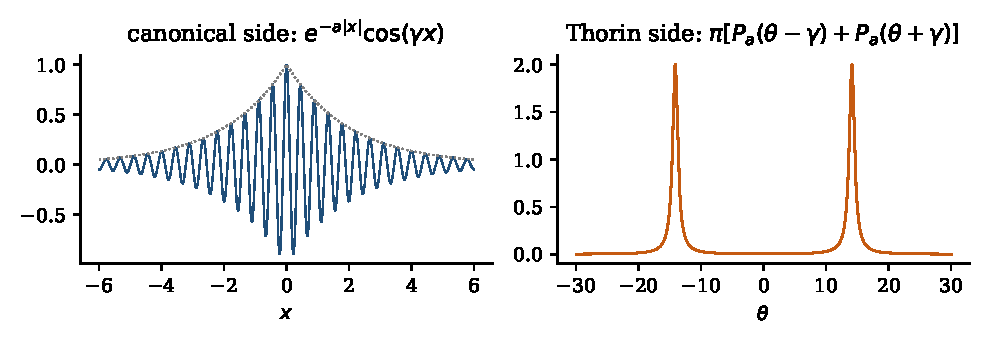
\includegraphics[width=\textwidth]{fig/cm_pair.pdf}
\caption{The reverse kernel for one zero, $a=\frac12$, $\gamma=\gamma_1$: a damped cosine on the canonical side and a Cauchy pair on the Thorin side (Lemma~\ref{cm:lem:kernel}). The damping rate is the width.}
\label{cm:fig:pair}
\end{figure}

\begin{theorem}\label{cm:thm:reverse}
Let $\alpha\ge1$, or more generally let $\alpha>\frac12$ with every zero having $\beta<\alpha$. The series $K_\alpha(x)=\sum_{\gamma>0}e^{-(\alpha-\beta)|x|}\cos\gamma x$ converges in $\mathcal S'(\R)$; its Fourier cosine transform is $v_\alpha$; on $(0,\infty)$ it equals $-\frac12xL_\alpha$, with $c=b_\alpha=\sum_\rho(\alpha-\rho)^{-1}$; and it is positive definite, with $v_\alpha>0$.
\end{theorem}

\begin{proof}
Each term is bounded by $1$, and two integrations by parts against a Schwartz function give $O(\gamma^{-2})$, the only boundary term coming from the kink at $0$; since $\sum\gamma^{-2}<\infty$ the series converges in $\mathcal S'$, and the transform follows term by term from Lemma~\ref{cm:lem:kernel} and Proposition~\ref{prop:struct}. The Hadamard product and Lemma~\ref{cm:lem:kernel} give $\log\xi(\alpha+s)/\xi(\alpha)=\int_0^\infty(1-e^{-sx})2K_\alpha(x)\,dx/x$, and $1-e^{-sx}=sx-(e^{-sx}+sx-1)$ identifies $L_\alpha=-2K_\alpha\,dx/x$ and $c$. Every width $\alpha-\beta$ is positive, so $v_\alpha>0$, and a tempered distribution with positive Fourier transform is positive definite.
\end{proof}

Read with the forward lemma, the canonical measure at $\alpha$ has two expressions, the primes with the archimedean and pole densities, and $-2\sum e^{-(\alpha-\beta)x}\cos\gamma x$ over the zeros. Their equality is the explicit formula.

\begin{theorem}\label{cm:thm:single}
Let $\alpha\ge1$. If $v_\alpha/\pi=P_{\alpha-1/2}*\nu$ for a positive measure $\nu$, so that the Thorin density of $1/\xi$ at the single basepoint $\alpha$ is a positive Cauchy mixture of the single width $\alpha-\frac12$, then RH holds, the P\'olya law is ferromagnetic, and $\nu=\sum_\gamma\delta_\gamma$. The converse holds at every $\alpha>\frac12$.
\end{theorem}

\begin{proof}
This is Theorem~\ref{tf:thm:deconv}(b). Put $H(t,\theta)=(P_{t-1/2}*\nu)(\theta)\ge0$, harmonic on $t>\frac12$. For $t>\alpha$, $v_t/\pi=P_{t-\alpha}*(v_\alpha/\pi)=H(t,\cdot)$ by the semigroup law. Both sides are harmonic on the connected set $\{t>\frac12\}$ minus the zeros, so they agree there, and a zero with $\beta>\frac12$ would make $v_t(\gamma)\to-\infty$ as $t\uparrow\beta$, against $H\ge0$.
\end{proof}

\begin{theorem}\label{cm:thm:weil}
Let $h$ be even and real with $e^{|x|/2}(|h|+|h''|)$ integrable, and $\alpha\ge1$, $w=\alpha-\frac12$. Group the zeros in pairs $\{\rho,1-\bar\rho\}$ with real parts $\frac12\pm\delta$, a zero on the line ($\delta=0$) forming a pair by itself, with the single term $e^{(\frac12-\alpha)|x|}$ in the sum below. Then
\[
\big\langle e^{w|x|}K_\alpha,h\big\rangle:=\sum_{\rm pairs}\int\big(e^{(\frac12+\delta-\alpha)|x|}+e^{(\frac12-\delta-\alpha)|x|}\big)e^{w|x|}\cos(\gamma x)h(x)\,dx=\frac12\sum_\rho\widehat h(t_\rho),
\]
with $t_\rho=(\rho-\frac12)/i$ and $\widehat h(t)=\int h(x)e^{-itx}dx$; the series converges absolutely and does not depend on $\alpha$. It is Weil's functional \cite{Weil52}; under RH it equals $\frac12\sum_\gamma|\widehat g(\gamma)|^2\ge0$ for $h=g*\tilde g$, and Weil's criterion gives the converse \cite{Weil52,Bombieri}.
\end{theorem}

\begin{proof}
Within a pair $e^{(\frac12\pm\delta-\alpha)|x|}e^{(\alpha-\frac12)|x|}=e^{\pm\delta|x|}$, whose sum $2\cosh\delta x$ is smooth, so the kink of $e^{w|x|}$ disappears pair by pair, and $\int2\cosh(\delta x)\cos(\gamma x)h=\widehat h(\gamma-i\delta)+\widehat h(\gamma+i\delta)$ for even $h$. The hypothesis on $h$ makes $\widehat h$ analytic on $|\im t|\le\frac12$ and $O(|\re t|^{-2})$ there, and $|\delta|<\frac12$.
\end{proof}

So the single width hypothesis, read on the canonical side, is Weil's criterion, and the place where the prime measure $\Lambda(n)n^{-\alpha}$ stops being tempered, $\alpha=1$, is removed by pairing each zero with its reflection: the kernel $\cosh\delta x$ grows at most like $e^{|x|/2}$. The windows of Weil positivity certified in Chapters~\ref{chap:wt} and following of Volume II are certificates for this functional on test functions of bounded support.

\section{The cosine tilted laws}\label{cm:sec:tilt}

For $w\ge0$ let $p_w=\cosh(wx)\,p/\E\cosh(wX)$. Its characteristic function is $\re\xi(\frac12+w+it)/\xi(\frac12+w)$.

\begin{theorem}\label{cm:thm:tilt}
For $X$ of Xi type and $w>0$, the law $\cosh(wx)\,P(dx)/\E\cosh(wX)$ is ferromagnetic whenever every zero of $L$ has $|\re r|<w$. In particular $p_w$ is ferromagnetic for every $w\ge\frac12$, with no hypothesis.
\end{theorem}

\begin{proof}
The moment generating function is proportional to $L(s+w)+L(s-w)$, and $|L(s-w)|=|L(w-y+iv)|$ at $s=y+iv$, since $L$ is even and real. A zero $r=\delta+i\gamma$ contributes $|w+y+iv-r|/|w-y+iv-r|$ to $|L(s+w)|/|L(s-w)|$, and $(w+y-\delta)^2-(w-y-\delta)^2=4y(w-\delta)>0$ for $y>0$; the partner $-r$ also has real part below $w$, and $e^{bs^2}$ contributes $e^{4bwy}\ge1$. So $|L(s+w)|>|L(s-w)|$ for $y>0$, and the sum has no zeros off the imaginary axis. For the P\'olya law $|\re r|=|\beta-\frac12|<\frac12$.
\end{proof}

In Thorin terms the comparison is $\log|L(w+y+iv)|-\log|L(w-y+iv)|=\pi\int_{w-y}^{w+y}u_t(v)\,dt$: the density is integrated across a horizontal segment centred at the level $w$, and each Cauchy bump contributes a positive amount as soon as its zero lies within $w$ of the axis. This is de Bruijn's lemma \cite[Lemma 1]{deBruijn}, the simplest case of Proposition~\ref{fm:prop:bruijn} and Theorem~\ref{pol:thm:cosh}(ii); Lagarias proved that the zeros of $\xi(s+w)+\xi(s-w)$ are simple for $w\ge\frac12$ \cite{Lagarias05}. With Theorem~\ref{fm:thm:closed}, RH holds if and only if $p_w$ is ferromagnetic for every $w>0$.

\begin{figure}[htbp]
\centering
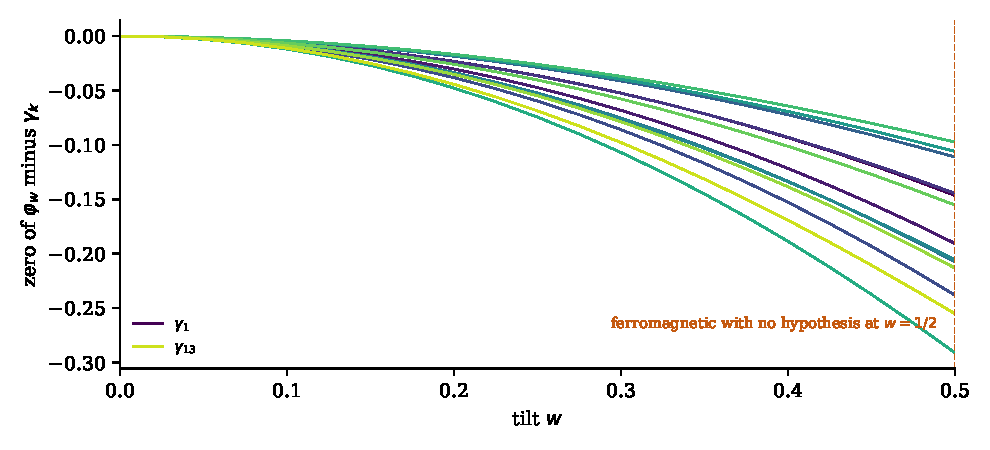
\includegraphics[width=\textwidth]{fig/cm_traj.pdf}
\caption{Zeros of the characteristic function of $p_w$ on $(0,60)$ minus $\gamma_k$, against $w$. They move continuously and stay real; at $w=\frac12$ the law is ferromagnetic with no hypothesis. The displacement is quadratic in $w$ for small $w$, as the first order rule of Remark~\ref{fm:rem:firstorder} predicts (computed).}
\label{cm:fig:traj}
\end{figure}

\section{A two spin Lee and Yang form of RH}\label{cm:sec:pair}

Let $\varepsilon$ be a fair sign independent of $X$ and couple the two spins with strength $w>0$. With fields $h_1$ on $X$ and $h_2$ on $\varepsilon$ the partition function is
\[
Z_w(h_1,h_2)=\E\sum_{\varepsilon=\pm1}e^{wX\varepsilon+h_1X+h_2\varepsilon}=e^{h_2}L(h_1+w)+e^{-h_2}L(h_1-w).
\]
The marginal law of $X$ is the cosine tilt, and the pair has the multivariate Lee and Yang property if $Z_w\ne0$ whenever $\re h_1>0$ and $\re h_2>0$.

\begin{theorem}\label{cm:thm:pair}
Let $X$ be of Xi type and $w>0$.
\begin{enumerate}
\item[(a)] If no zero of $L$ has $\re r>w$, the pair has the Lee and Yang property.
\item[(b)] If the pair has the Lee and Yang property, no zero of $L$ has $\re r>w$. So the pair has the Lee and Yang property at the coupling $w$ exactly when $X\in\mathcal C_w$.
\item[(c)] For $w_0\ge0$, the pair has the Lee and Yang property for every $w>w_0$ if and only if no zero has $\re r>w_0$.
\end{enumerate}
\end{theorem}

\begin{proof}
A zero of $Z_w$ solves $e^{2h_2}=g(h_1)$ with $g=-L(h_1-w)/L(h_1+w)$, and $e^{2h_2}$ ranges over $\{|z|>1\}$ when $\re h_2>0$; so the property is $|g|\le1$ on $\re h_1>0$, poles excluded. (a) is the factor comparison of Theorem~\ref{cm:thm:tilt}, in which a zero with $\re r=w$ contributes the ratio $1$, so $|g|\le1$. (b) Let $r$ be a zero with $\re r>w$ and put $h_1=r-w$, so $\re h_1>0$. If $L(r-2w)=0$, then $Z_w(h_1,h_2)=0$ for every $h_2$; otherwise $g$ has a pole at $h_1$ and takes every large modulus near it. Either way the property fails. (c) follows from (a) and (b).
\end{proof}

\begin{corollary}\label{cm:cor:pair}
The P\'olya spin coupled to one Ising spin with coupling $w$ is a Lee and Yang ferromagnet for every $w\ge\frac12$, with no hypothesis. For $w_0\in[0,\frac12)$ it is one for every $w>w_0$ if and only if $\zeta$ has no zero with $\re s>\frac12+w_0$. RH holds if and only if it is one for every $w>0$; under the announced half plane at $\frac78$, for every $w>\frac38$.
\end{corollary}

\begin{proposition}\label{cm:prop:euler}
For $N\ge2$ let $E_N(s)=\prod_{p\le N}(1-p^{-1/2-s})(1-p^{-1/2+s})$, the truncated Euler product of $\zeta(\frac12+s)^{-1}\zeta(\frac12-s)^{-1}$. Its zeros are $\pm\frac12+2\pi ik/\log p$, and the two spin system built from $E_N$ in place of $L$ has the Lee and Yang property exactly for $w\ge\frac12$.
\end{proposition}

\begin{proof}
$(1-p^{-1/2-s})(1-p^{-1/2+s})=1+p^{-1}-2p^{-1/2}\cosh(s\log p)$ vanishes exactly when $\cosh(s\log p)=\cosh(\frac12\log p)$. $E_N$ is even, real and of exponential type, with Hadamard product $E_N(0)\prod(1-s^2/r^2)$ and $\sum|r|^{-2}<\infty$, so Theorem~\ref{cm:thm:pair} applies to it as an entire function. For $w>\frac12$ part (a) applies; at $w=\frac12$ the zeros with $\re r=\frac12$ contribute factor ratios equal to $1$ and their partners ratios above $1$, so $|g|<1$ still. For $w<\frac12$ the zeros with $\re r=\frac12>w$ violate part (b).
\end{proof}

So finite Euler products sit exactly at the coupling $\frac12$, the line $\re s=1$, which is where the P\'olya law reaches unconditionally; the symmetrised infinite product converges absolutely nowhere. Coupling below $\frac12$ needs the cancellation of the infinite product, which is the zero free region problem.

\section{The one variable test is weaker}\label{cm:sec:counter}

Theorem~\ref{cm:thm:tilt} gives ferromagnetism of the cosine tilt from the strip. The converse fails for the one variable tilt (Proposition~\ref{cm:prop:twospin}), although it holds for the pair by Theorem~\ref{cm:thm:pair}.

In two exact models the threshold is the strip. For $X\in\{-1,0,1\}$ with $P(X=\pm1)=q<\frac14$, $L(s)=(1-2q)+2q\cosh s$ has zeros at real parts $\pm a$, $\cosh a=\frac{1-2q}{2q}$, and the tilt $2(1-2q)+4q\cosh s\cosh w$ is ferromagnetic exactly for $w\ge a$ (proved). For $qU_1+(1-q)U_3$ with $q>\frac14$, $U_c$ uniform on $[-c,c]$, the nonreal zeros sit at $\pm i\delta$ from the real axis with $\delta=\operatorname{arccosh}\sqrt{3/(4(1-q))}$; counting by the argument principle in $|\re|\le40\pi+0.37$, $|\im|\le4$, all $160$ nonreal zeros are gone from $w=\delta+0.002$ on, and a few become real just before $\delta$ ($152$ of $160$ remain at $w=\delta-0.002$ for $q=\frac12$; computed).

The first model has a sum of two independent copies that is a sharper example, because there the threshold lies strictly inside the strip.

\begin{proposition}[the sum of two three point spins]\label{cm:prop:twospin}
Let $0<q<\frac14$, $\cosh a=\frac{1-2q}{2q}$ (so $a>0$), and $X=Y_1+Y_2$ with $Y_1,Y_2$ independent and $P(Y_i=\pm1)=q$, $P(Y_i=0)=1-2q$. Then $X$ is of Xi type, and its cosine tilt is ferromagnetic exactly for $w\ge w^*$, where $\cosh 2w^*=\cosh^2a$. Moreover $\sinh w^*=\sinh a/\sqrt2$, $a/\sqrt2<w^*<a$, and $w^*/a\to\cos\frac\pi4$ as $q\uparrow\frac14$. Since $L$ has its zeros at real parts $\pm a$, $X$ lies in $\mathcal C_a$ and not in $\mathcal C_w$ for $w<a$. So for every $w\in[w^*,a)$ the cosine tilt of $X$ at $w$ is ferromagnetic while $X\notin\mathcal C_w$. For $w>0$ and $w<w^*$ the tilt has no zero on the imaginary axis at all. (Proved.)
\end{proposition}

\begin{proof}
Put $A=\cosh a$. Then $L(s)=\E e^{sX}=(1-2q+2q\cosh s)^2=4q^2(A+\cosh s)^2$, an even entire function of order one with zeros at $\cosh s=-A$, that is $s=\pm a+i\pi(2k+1)$, double, so $X$ is of Xi type and $X\in\mathcal C_a\setminus\mathcal C_w$ for $w<a$. The moment generating function of the tilted law is a multiple of $M_w(s)=L(s+w)+L(s-w)$, so ferromagnetism at $w$ means that every zero of $M_w$ has $\re s=0$. Write $c=\cosh s$, $C=\cosh w$, $S=\sinh w$. As $\cosh(s\pm w)=cC\pm S\sinh s$ and $\sinh^2s=c^2-1$,
\[
M_w(s)=8q^2Q_w(\cosh s),\qquad Q_w(c)=\cosh(2w)\,c^2+2AC\,c+A^2-S^2 .
\]
Since $\cosh$ maps $\mathbb C$ onto $\mathbb C$, and $\cosh s\in[-1,1]$ exactly when $\re s=0$ (for $s=x+iy$, $\cosh s=\cosh x\cos y+i\sinh x\sin y$, and $|\cosh s|=\cosh x>1$ if $x\ne0$ and $\cosh s$ is real), the zeros of $M_w$ lie on the axis exactly when both roots $c_\pm$ of $Q_w$ lie in $[-1,1]$, and none lies on the axis when neither does. The discriminant of $Q_w$ is
\[
(AC)^2-(C^2+S^2)(A^2-S^2)=\sinh^2w\,(\cosh2w-\cosh^2a),
\]
which for $w>0$ is negative, zero or positive according as $w<w^*$, $w=w^*$ or $w>w^*$.

If $0<w<w^*$ the roots are $c_\pm=(-AC\pm iS\sqrt{\cosh^2a-\cosh2w})/\cosh2w$, not real because $S>0$, so $M_w$ has zeros, and none on the axis.

If $w>w^*$ the roots are real, $c_-\le c_+$. Here $Q_w(1)=(C+A)^2>0$ and $Q_w(-1)=(C-A)^2\ge0$, and the vertex $c_0=-AC/\cosh2w$ satisfies $-1\le c_0<0$: from $\cosh 2w\ge A^2$ we get $A\le\sqrt{2C^2-1}$, and $C\sqrt{2C^2-1}\le2C^2-1$ because $C\ge1$, so $0<AC\le\cosh 2w$. If $c_-<-1$, then $Q_w(-1)\ge0$ would force $c_+\le-1$ as well, so $c_0<-1$, a contradiction; so $c_-\ge-1$. As $Q_w(1)>0$, both roots lie on the same side of $1$, and both above $1$ would put $c_0>1$; so $c_+<1$. Hence $c_\pm\in[-1,1)$ and every zero is on the axis.

If $w=w^*$ the root is double, $c_0=-C/A$. Since $C^2=(1+A^2)/2<A^2$ for $A>1$, we have $c_0\in(-1,0)$ and all zeros are on the axis (each of multiplicity two).

Finally $\cosh 2w^*=\cosh^2a$ reads $\sinh w^*=\sinh a/\sqrt2$, so $w^*<a$; and $\sinh x/x$ is increasing on $(0,\infty)$, so $\sinh(a/\sqrt2)<\sinh a/\sqrt2=\sinh w^*$, which gives $w^*>a/\sqrt2$. As $q\uparrow\frac14$, $A\downarrow1$ and $a\downarrow0$, and $w^*/a=\frac{\operatorname{arsinh}u}{u}\cdot\frac{\sinh a}{a}\cdot\frac1{\sqrt2}\to\frac1{\sqrt2}$ with $u=\sinh a/\sqrt2\to 0$.
\end{proof}

For $q=0.2$ ($a=0.9624$) the threshold is $w^*=0.7253$. The ratio $w^*/a$ is $0.7536$, $0.7165$, $0.7080$ and $0.70720$ at $q=0.2$, $0.24$, $0.249$ and $0.2499$ (computed).

Plant a pair off the line in $\Xi$: with $c=\frac12(\gamma_k+\gamma_{k+1})+i\eta$ let
\[
F(z)=\Xi(z)\,\frac{(z^2-c^2)(z^2-\bar c^2)}{(z^2-\gamma_k^2)(z^2-\gamma_{k+1}^2)},
\]
an even entire function, real on the real axis, with strip half width $\eta$.

\begin{proposition}\label{cm:prop:counter}
For $k=1$ and $\eta=0.3$, $F(z+iw)+F(z-iw)$ has only real zeros in $[1,45.3]\times[-2.2,2.2]$ at $w=0.299<\eta$. The nonreal zero born from $c$ reaches the real axis at $w^*\approx0.2951$, its imaginary part behaving like $(w^*-w)^{1/2}$. The inverse Fourier transform of $F$ is positive at $x=0,0.25,\dots,1.25$, with ratio to the P\'olya density between $0.989$ and $1.111$ (computed, floating point).
\end{proposition}

The exact law of Proposition~\ref{cm:prop:twospin} proves unconditionally that ferromagnetism of the cosine tilt at $w$ does not force a law of Xi type into $\mathcal C_w$, for every $w\in[w^*,a)$. The planted computation illustrates the same fact for $\Xi$: if the planted density is positive on $\R$ and the tilt has no nonreal zero outside the box (which needs the zeros of $\zeta$ above height $45.3$ to lie close to the line, for instance RH), ferromagnetism of the cosine tilt at $w$ does not force $\Xi$ with the planted pair into $\mathcal C_w$; the two variable property of Theorem~\ref{cm:thm:pair} is needed. Table~\ref{cm:tab:survey} repeats the computation for planted pairs at other heights and widths.

\begin{table}[htbp]
\centering\small
\begin{tabular}{rrcccc}
\toprule
$k$ & height $m$ & $\eta=0.1$ & $\eta=0.2$ & $\eta=0.3$ & $\eta=0.4$\\
\midrule
$1$ & $17.58$ & $0.0998$ & $0.1985$ & $0.2951$ & $0.3888$\\
$3$ & $27.72$ & $0.0997$ & $0.1980$ & $0.2935$ & $0.3854$\\
$5$ & $35.26$ & $0.0997$ & $0.1983$ & $0.2944$ & $0.3873$\\
$8$ & $45.67$ & $0.0997$ & $0.1978$ & $0.2928$ & $0.3839$\\
$11$ & $54.71$ & $0.0997$ & $0.1978$ & $0.2929$ & $0.3842$\\
$15$ & $66.10$ & $0.0996$ & $0.1971$ & $0.2907$ & $0.3796$\\
\bottomrule
\end{tabular}
\caption{Slice thresholds $w^*$ for $\Xi$ with the ordinates $\gamma_k,\gamma_{k+1}$ replaced by the pair $m\pm i\eta$, $m=\frac12(\gamma_k+\gamma_{k+1})$: the least $w$ at which the nonreal zero born from $m+i\eta$ reaches the real axis, found by continuation in $w$ (computed, mpmath at 15 digits, floating point). Every threshold lies below $\eta$, as Theorem~\ref{cm:thm:tilt} requires, and the gap $\eta-w^*$ is close to $C\eta^3$ with $C$ between $0.17$ and $0.38$, larger at the later ordinates of the table (the run to height $10^4$ below shows that $C=\frac12\phi^2$ then saturates and fluctuates).}
\label{cm:tab:survey}
\end{table}

In every case the gap is of third order in the width (computed; Theorem~\ref{cm:thm:exact} proves the law $\eta-w^*\sim C\eta^3$ as $\eta\to0$, with $C=\frac12\phi^2$). So the one variable test measures the strip up to a small third order error, and it is not exact: a law can pass it at a coupling below its Cauchy defect (Proposition~\ref{cm:prop:twospin}, proved, and for $\Xi$ with a planted pair Proposition~\ref{cm:prop:counter}, conditionally).

\begin{figure}[htbp]
\centering
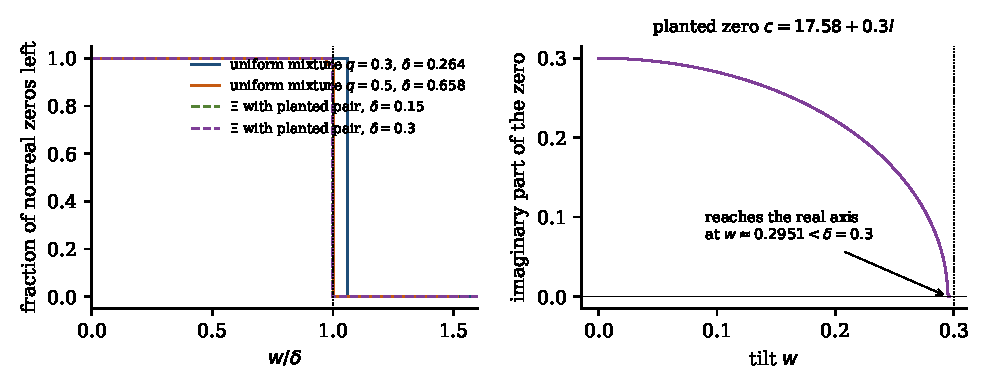
\includegraphics[width=\textwidth]{fig/cm_threshold.pdf}
\caption{Left: fraction of nonreal zeros remaining after the cosine tilt, against $w/\delta$, for two uniform mixtures and for $\Xi$ with a planted pair. Right: imaginary part of the zero born from the planted zero $17.58+0.3i$, which reaches the real axis at $w\approx0.2951<\delta$ (computed).}
\label{cm:fig:threshold}
\end{figure}

The mechanism is a phase criterion. For real $x$, $F(x-iw)=\overline{F(x+iw)}$, so the tilt is $2\re F(x+iw)$ on the real axis.

\begin{proposition}\label{cm:prop:phase}
Let $\Theta_w(x)$ be a continuous argument of $F(x+iw)$ on an interval $I$ where $F(x+iw)\ne0$. The real zeros of the tilt in $I$ are the points where $\Theta_w\in\frac\pi2+\pi\mathbb Z$. A real zero $a$ of $F$ contributes $\arg(x-a+iw)$ to $\Theta_w$, which decreases by $\pi$ across $a$; a zero $c=m+i\eta$ contributes $\arg(x-m+i(w-\eta))$, which increases by $\pi$ across $m$ when $w<\eta$ and decreases when $w>\eta$, while $\bar c$ contributes a decrease. So for $w<\eta$ the planted pair produces a local rise of $\Theta_w$ near $m$, of height tending to $\pi$ as $w\uparrow\eta$, and two nonreal zeros of the tilt become real exactly when that rise first reaches a level $\frac\pi2+k\pi$.
\end{proposition}

\begin{proof}
On the real axis the tilt is $2|F(x+iw)|\cos\Theta_w(x)$. The contributions are those of the factors of the Hadamard product of $F$. The total number of zeros of the tilt in a rectangle around $I$ is constant in $w$ as long as none crosses its boundary, so a pair of real zeros appears exactly when a pair of nonreal ones disappears; and a new pair of real zeros appears exactly when a local maximum of $\Theta_w$ reaches a level $\frac\pi2+k\pi$.
\end{proof}

Whether the rise reaches the level before $w=\eta$ depends on where the background phase of the other zeros puts the level, so the slice threshold can lie below the strip by an amount that depends on the configuration, and it can never lie above it (Theorem~\ref{cm:thm:tilt}). Figure~\ref{cm:fig:phase} shows the rise touching the level $\frac32\pi$ at $w\approx0.2951$.

\begin{figure}[htbp]
\centering
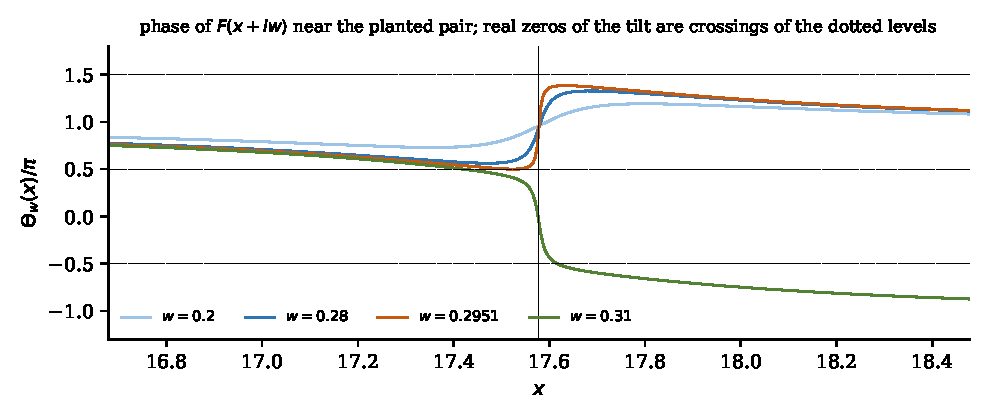
\includegraphics[width=\textwidth]{fig/cm_phase.pdf}
\caption{The phase $\Theta_w$ near the planted pair of Proposition~\ref{cm:prop:counter}. For $w<0.2951$ the local rise stays below the level $\frac32$; at $w\approx0.2951$ it touches it, and two real zeros appear; for $w>\eta=0.3$ the phase drops by about $2\pi$ (computed).}
\label{cm:fig:phase}
\end{figure}

\section{The size of the gap}\label{cm:sec:gap}

The phase criterion has an exact form. Write $G=F/((z-c)(z-\bar c))$ for $F$ without the planted pair $c=m+i\eta$, $\bar c$; it keeps the mirror pair $-c,-\bar c$ and the real zeros, it is real on the real axis, and we assume $G(m)\ne0$. For $0<w<\eta$ and real $x=m+u$, the two factors of the pair combine:
\[
\arg\big((u+iw-i\eta)(u+iw+i\eta)\big)=\arg\big(u^2+\eta^2-w^2+2iwu\big)=\arctan\frac{2wu}{u^2+\eta^2-w^2},
\]
the principal value, since the real part is positive. Put $\psi_w(x)=\arg G(x+iw)$, a continuous branch near $m$.

\begin{theorem}\label{cm:thm:exact}
Let $r>0$ be such that $G$ has no zero in the disc $|z-m|\le2r$. For $\eta$ small enough the tilt $F(z+iw)+F(z-iw)$ has exactly two zeros in $|z-m|<r$ for every $w\in(0,\eta)$, and they are real if and only if
\[
\Phi_w(u)=\arctan\frac{2wu}{u^2+\eta^2-w^2}+\psi_w(m+u)
\]
takes a value in $\frac\pi2+\pi\mathbb Z$ for some $u\in(-r,r)$. If $\phi=(G'/G)(m)\ne0$, the slice threshold satisfies
\[
\eta-w^*=\tfrac12\,\phi^2\,\eta^3\big(1+O(\eta)\big)\qquad(\eta\to0),
\]
and if $\phi=0$, then $\eta-w^*=O(\eta^7)$.
\end{theorem}

\begin{proof}
As $\eta\to0$, uniformly in $w\in[0,\eta]$, the tilt converges on $|z-m|\le r$ to $2(z-m)^2G(z)$, with $G$ read as its limit as $\eta\to0$, which has a double zero at $m$ and no other zero there; by Hurwitz's theorem the tilt has exactly two zeros in $|z-m|<r$ for $\eta$ small. Nonreal zeros come in conjugate pairs, so the two are both real or both nonreal. On the real axis $F(x-iw)=\overline{F(x+iw)}$, so the tilt is $2|F(x+iw)|\cos\arg F(x+iw)$, and $\arg F(x+iw)=\Phi_w(x-m)$ by the display above; real zeros are the points where $\Phi_w\in\frac\pi2+\pi\mathbb Z$.

For the asymptotics write $w=\eta-\varepsilon$ and $a=(\eta^2-w^2)^{1/2}$. The first term of $\Phi_w$ is odd in $u$, with extreme values $\pm\arcsin(w/\eta)$ at $u=\pm a$, and it is $O(w/|u|)$ for $|u|\gg a$. Since $G$ is real on the real axis, $\psi_w(m)=w\phi+O(w^3)$ modulo $\pi$ and $\psi_w'(m+u)=\im(G'/G)(m+u+iw)=O(w)$. Suppose $\phi>0$; the case $\phi<0$ is the mirror image with the level $-\frac\pi2$. Then $\Phi_w$ stays above $-\frac\pi2$, and its maximum is $\psi_w(m)+\arcsin(w/\eta)+O(\eta a)$, attained near $u=a$. It reaches $\frac\pi2$ exactly when $\arccos(w/\eta)\le\psi_w(m)+O(\eta a)$. Here $\arccos(w/\eta)=(2\varepsilon/\eta)^{1/2}(1+O(\varepsilon/\eta))$ and $a=(2\eta\varepsilon)^{1/2}(1+O(\varepsilon/\eta))$. At the threshold $\varepsilon$ is of order $\eta^3$, so $\eta a=O(\eta^3)$, while $\psi_w(m)=\eta\phi(1+O(\eta))$; hence $(2\varepsilon^*/\eta)^{1/2}=\eta\phi(1+O(\eta))$, which is the stated law. If $\phi=0$, then $\psi_w(m)=O(\eta^3)$, the same comparison gives $(2\varepsilon^*/\eta)^{1/2}=O(\eta^3)$, and $\varepsilon^*=O(\eta^7)$.
\end{proof}

The coefficient is the field that all the other zeros exert at the planted pair,
\[
\phi(m)=\frac{G'}G(m)=\sum_a\frac1{m-a}+\frac{4m}{4m^2+\eta^2},
\]
the sum over the real zeros of $F$ in symmetric pairs and the last term from the mirror pair; it grows over the first ordinates, as the constants of Table~\ref{cm:tab:survey} do ($\phi=-0.62$ at $k=1$, $-0.88$ at $k=15$), and then saturates and fluctuates (see the run to height $10^4$ below). The exact criterion reproduces the thresholds found by continuation to every printed digit: for $k=1,3,8,15$ and $\eta=0.1,0.3$ it gives $0.099810$, $0.295090$, $0.099746$, $0.293544$, $0.099711$, $0.292783$, $0.099619$ and $0.290699$, against $0.09981$, $0.29509$, $0.09975$, $0.29354$, $0.09971$, $0.29278$, $0.09962$ and $0.29069$ (computed).

\begin{remark}[heuristic]\label{cm:prop:gap}
Solved as a fixed point with the cubic and quadratic terms kept, the criterion gives
\[
\varepsilon^*=\frac{\operatorname{dist}\big(\arg G(m+iw^*),\pi\mathbb Z\big)^2}{4\big(b+\frac1{2\eta-\varepsilon^*}\big)},\qquad b=-\im\frac{G'}G(m+iw^*),
\]
to the order of Theorem~\ref{cm:thm:exact}.
\end{remark}

Two further computations test it.

First, solved as a fixed point, this formula reproduces all twenty four thresholds of Table~\ref{cm:tab:survey} to within about $1.5\%$, which is the resolution of the table, at every height and width (Figure~\ref{cm:fig:round3}, left; computed). An earlier version that left out the mirror pair was off by up to $18\%$ at the first pair; the term $4m/(4m^2+\eta^2)\approx1/m$ is what matters at low height.

Second, the formula predicts that a pair planted where $\phi$ vanishes has a gap of much higher order. For $k=3$ and $k=5$ we located the zero of $\phi$ in the gap left by the removed ordinates, at $m=22.961$ and $m=32.156$, and planted the pair there. The gaps fell from $2.5\times10^{-4}$ and $2.2\times10^{-4}$ at the midpoint to $1.2\times10^{-9}$ at $\eta=0.1$, and from $1.5\times10^{-2}$ and $1.3\times10^{-2}$ to $1.5\times10^{-6}$ and $2.8\times10^{-6}$ at $\eta=0.4$, a reduction by four to five orders of magnitude. Between $\eta=0.2$ and $\eta=0.4$ they grow by factors of $100$ and $110$, close to the factor $2^7=128$ of an $\eta^7$ law (Figure~\ref{cm:fig:round3}, centre; computed, thresholds resolved to about $10^{-9}$).

So the one variable test misses the strip by an amount set by a single local quantity, the field of the other zeros at the pair: by $\frac12\phi^2\eta^3$, and by almost nothing where the field vanishes.

\paragraph{The field and the thresholds to height $10^4$ (computed, with ball arithmetic where stated).} The field was evaluated for the midpoint pair ($\eta=0.1$) at each of the first $10^4$ ordinates, with the ordinates $\gamma_k$ as the balls of the certified zero enumeration of \texttt{acb.zeta\_zeros} and every value a ball of radius below $3\times10^{-31}$ (128 bit). The field is negative for $93.0\%$ of the pairs, with mean $-0.785$ and standard deviation $0.531$; it does not keep growing. By decade of height the mean is $-0.736$, $-0.781$, $-0.784$, $-0.785$, $-0.786$ and the median of $|\phi|$ is $0.78$ at every height, while only the spread grows ($0.12$ below height $100$, $0.58$ above $6000$). Values at later ordinates are $-1.017$ at $k=100$, $-0.396$ at $k=1000$, $-0.354$ at $k=3000$ and $-0.692$ at $k=9999$. Small values are rare: $|\phi|<10^{-2}$ for $43$ of the $10^4$ pairs ($0.43\%$, none below height $1000$) and $|\phi|<0.1$ for $4.8\%$. For every $k$ the field as a function of the position of the pair has exactly one sign change in the window $(\gamma_{k-1},\gamma_{k+2})$ (grid and bisection, computed), and about $0.3\%$ of the window lies within $10^{-2}$ of it.

The slice thresholds were recomputed by the exact criterion of Theorem~\ref{cm:thm:exact} (flint, 160 bit balls for the criterion, double precision for the argument) for $k$ up to $9999$ at $\eta=0.1$ and $0.3$. The eight values above are reproduced to six digits. The ratio of the measured gap to $\frac12\phi^2\eta^3$ falls from $0.995$ at $k=1$ to $0.951$ at $k=9999$ for $\eta=0.1$, and from $0.954$ to $0.688$ for $\eta=0.3$, the $O(\eta)$ correction being larger where the zeros are denser. The fixed point of Remark~\ref{cm:prop:gap} reproduces the gap to $0.2\%$ at $\eta=0.1$ and $1.2\%$ at $\eta=0.3$ for every $k$ run. At the zero of the field ($|\phi|<3\times10^{-12}$) the gap at $\eta=0.1$ is $1.9\times10^{-10}$ to $1.6\times10^{-9}$, which is $1.7\times10^4$ to $2.3\times10^6$ times smaller than at the midpoint, and from $\eta=0.1$ to $0.3$ it grows by $1984$, $1905$, $1540$, $1666$ and $1499$ for $k=8$, $100$, $1000$, $3000$ and $9999$, against $3^7=2187$ for an $\eta^7$ law.

{\emergencystretch=4em The two spin test was run as a zero free rectangle. In the three windows $[10.0,109.1]$, $[1000.6,1100.0]$ and $[9792.9,9878.2]$ (33, 81 and 100 zeros), the rectangle $w\le\operatorname{Im}z\le1.5$ over the window contains no zero of $\Xi$ for each $w=0.5,0.4,0.3,0.2,0.1,0.05$: the winding number of $\Xi$ around the boundary in 96 bit ball arithmetic is $0$ in all $18$ cases (certified, apart from the Euler product bound at $\sigma=2$, which was not computed). This is the zero free region of the window for the pair, not the global property of Corollary~\ref{cm:cor:pair}. The one variable test on the same windows (every zero of $\Xi(z+iw)+\Xi(z-iw)$ in $|\operatorname{Im}z|\le1$ real, by the same winding routine and the sign changes on a grid of step $0.04$) passes in all $18$ cases and costs $13$ to $18$ thousand evaluations of $\Xi$, nearly independent of $w$. The cost of the rectangle grows like $1/w$ times the width of the window: relative to the one variable test, $0.33$, $0.62$ and $1.0$ at $w=0.5$ for the three windows, and $0.72$, $2.9$ and $9.9$ at $w=0.05$ ($165$ against $18$ seconds at height $10^4$). It is no dearer than the one variable test down to $w$ about $0.3$.\par}

Where the two tests differ the run shows it. For pairs planted at $k=8$ and $300$ ($\eta=0.3$) and $k=1000$ and $9999$ ($\eta=0.1$), with $w$ just above the threshold of the one variable test and below $\eta$ ($w=0.296391$, $0.297784$, $0.099962$ and $0.099886$), the one variable test passes (all $6$, $13$, $14$ and $16$ zeros real) while the rectangle contains the planted zero (count $1$); below the threshold the one variable test fails, and for $w>\eta$ both are clean. At $k=1000$ the rectangle detects the pair at $w=\eta-3.8\times10^{-5}$, so the two spin form loses nothing to the gap. This is a test on windows and on planted pairs, and it proves nothing about the zeros of $\zeta$ outside them.

\section{Several pairs and multiple zeros}\label{cm:sec:several}

The proof of Theorem~\ref{cm:thm:exact} is local, and it extends to configurations with several pairs off the line and to pairs of higher multiplicity. The answer has two parts. Each cluster of zeros off the line is seen by the one variable test separately, through its own field, which now includes the other clusters. And a multiple zero changes the order of the gap: a double pair is seen only at a fixed fraction of its distance from the line.

Fix distinct heights $m_1,\dots,m_K>0$, multiplicities $n_j\ge1$ and ratios $t_j\in(0,1]$, and let
\[
F=G_0\prod_{j=1}^K\big((z^2-c_j^2)(z^2-\bar c_j^2)\big)^{n_j},\qquad c_j=m_j+i\eta_j,\quad \eta_j=t_j\eta,
\]
with $G_0$ real entire, real on the real axis, and $G_0(m_j)\ne0$. Let $G_j=F/((z-c_j)(z-\bar c_j))^{n_j}$; as $\eta\to0$ it converges near $m_j$ to the function $G_j^0$ in which every other cluster has become a real zero of multiplicity $2n_l$ at $m_l$, so its field
\[
\phi_j=\frac{(G_j^0)'}{G_j^0}(m_j)=\frac{G_0'}{G_0}(m_j)+\sum_{l\ne j}\frac{2n_l}{m_j-m_l}+\sum_{l}\frac{2n_l}{m_j+m_l}
\]
contains the other clusters and all the mirror images. The local slice threshold $w_j^*$ is the least $w$ for which all $2n_j$ zeros of the tilt born from $c_j$ and $\bar c_j$ are real.

\begin{theorem}\label{cm:thm:several}
Let $r>0$ be such that $G_j^0$ has no zero in $|z-m_j|\le2r$ for every $j$. For $\eta$ small enough the tilt $F(z+iw)+F(z-iw)$ has exactly $2n_j$ zeros in $|z-m_j|<r$ for every $w\in[0,\eta]$; they are all real for $w\ge\eta_j$, and
\begin{enumerate}
\item for $n_j$ odd, $\eta_j-w_j^*=\frac{\phi_j^2}{2n_j^2}\,\eta_j^3\big(1+O(\eta)\big)$ when $\phi_j\ne0$, and $O(\eta^7)$ when $\phi_j=0$;
\item for $n_j$ even, $w_j^*=\eta_j\cos\frac\pi{2n_j}+O(\eta^2)$, and more precisely $w_j^*=\eta_j\sin\big(\frac{(n_j-1)\pi}{2n_j}+\frac{|\psi_j|}{n_j}\big)+O(\eta^3)$ with $\psi_j=\operatorname{dist}(\arg G_j(m_j+iw_j^*),\pi\mathbb Z)=O(\eta)$.
\end{enumerate}
The configuration is seen by the one variable test, in the sense that every zero born from a planted zero is real, exactly for $w\ge\max_jw_j^*$.
\end{theorem}

\begin{proof}
Fix $j$ and drop the index. As $\eta\to0$, uniformly in $w\in[0,\eta]$, the tilt converges on $|z-m|\le r$ to $2(z-m)^{2n}G^0(z)$, so by Hurwitz's theorem it has exactly $2n$ zeros there. On the real axis the tilt is $2|F(x+iw)|\cos\arg F(x+iw)$ and, with $x=m+u$ and $a^2=\eta^2-w^2$,
\[
\arg F(x+iw)=\Phi(u)=n\,A(u)+\psi_w(m+u),\qquad A(u)=\arg\big(u^2+a^2+2iwu\big),
\]
where $\psi_w=\arg G(\cdot+iw)$ varies by $O(\eta r)$ on $(-r,r)$, with derivative $O(\eta)$.

For $w<\eta$ the function $A$ is odd, decreases from $O(\eta/r)$ at $u=-r$ to $-\alpha$ at $u=-a$, increases to $\alpha$ at $u=a$ and decreases to $O(\eta/r)$ at $u=r$, with $\alpha=\arcsin(w/\eta)$. Put $\psi_0=\psi_w(m)$, taken in $(-\frac\pi2,\frac\pi2)$, so $\psi_0=O(\eta)$. Up to the error terms, $\Phi$ therefore passes once through every level of $\frac\pi2+\pi\mathbb Z$ in $(\psi_0-n\alpha,\psi_0)$ on $(-r,-a)$, once through every level in $(\psi_0-n\alpha,\psi_0+n\alpha)$ on $(-a,a)$, and once through every level in $(\psi_0,\psi_0+n\alpha)$ on $(a,r)$. So the number of real zeros is twice the number of levels in $(\psi_0-n\alpha,\psi_0+n\alpha)$, an interval of length $2n\alpha<n\pi$, which contains at most $n$ levels. All $2n$ zeros are real exactly when it contains $n$ of them. For $n$ even the levels needed are $\pm\frac\pi2,\dots,\pm\frac{(n-1)\pi}2$, and the condition is $n\alpha\ge\frac{(n-1)\pi}2+|\psi_0|$, which is the formula of (ii). For $n$ odd one side needs the level $\frac{n\pi}2$, and the condition is $n\alpha+|\psi_0|\ge\frac{n\pi}2$, that is $n\arccos(w/\eta)\le|\psi_0|$; with $\psi_0=\eta\phi(1+O(\eta))$ and $\arccos(w/\eta)=(2\varepsilon/\eta)^{1/2}(1+O(\varepsilon/\eta))$, $\varepsilon=\eta-w$, this is (i), exactly as in the proof of Theorem~\ref{cm:thm:exact}. The error terms are those of that proof: near the extrema $\psi_w$ moves by $O(\eta a)$, which is $O(\eta^3)$ at the threshold for $n$ odd and $O(\eta^2)$ for $n$ even, giving the stated orders.

For $w\ge\eta$ the real part of $u^2+a^2+2iwu$ is negative near $u=0$ and its imaginary part changes sign there, so $A$ decreases continuously by $2\pi-O(\eta/r)$ across $(-r,r)$ and $\Phi$ decreases by $2n\pi-O(\eta)$. It passes through at least $2n-1$ levels, hence, since nonreal zeros come in conjugate pairs and there are $2n$ zeros in all, through $2n$, and all the zeros are real. The last statement collects the clusters.
\end{proof}

Three consequences are worth recording.

First, the other clusters enter only through the field. A neighbour at distance $d$ adds $\pm2/d$ to $\phi_j$; it can enlarge the gap, and it can also cancel the field of the real zeros and hide the pair almost completely. Table~\ref{cm:tab:pairs} shows both, for two pairs of equal width planted in the gap left by $\gamma_8$ and $\gamma_9$, at $M\mp\frac d2$ with $M=\frac12(\gamma_8+\gamma_9)$. At $d=2$ the field at the upper pair is $0.037$ and its gap $6.5\times10^{-7}$, about $450$ times below that of a single pair at the same width. The fixed point of Remark~\ref{cm:prop:gap}, with $G_j$ in place of $G$, predicts every gap of two pairs of equal width with $d\ge0.3$ to within $7\%$, and to within $3\%$ for $d\ge1.2$, at widths $0.1$ and $0.2$, including separations of three times the width, where the theorem does not apply.

\begin{table}[htbp]
\centering
\begin{tabular}{cccccc}
$d$ & $\eta$ & pair & $\phi_j$ & gap $\eta-w_j^*$ & fixed point \\ \hline
$3.0$ & $0.1$ & lower & $-1.096$ & $5.88\times10^{-4}$ & $5.86\times10^{-4}$\\
$3.0$ & $0.1$ & upper & $-0.425$ & $8.92\times10^{-5}$ & $8.92\times10^{-5}$\\
$2.0$ & $0.1$ & lower & $-1.536$ & $1.13\times10^{-3}$ & $1.13\times10^{-3}$\\
$2.0$ & $0.1$ & upper & $+0.037$ & $6.47\times10^{-7}$ & $6.47\times10^{-7}$\\
$0.8$ & $0.1$ & lower & $-3.123$ & $4.18\times10^{-3}$ & $4.12\times10^{-3}$\\
$0.8$ & $0.1$ & upper & $+1.636$ & $1.21\times10^{-3}$ & $1.21\times10^{-3}$\\
$0.3$ & $0.1$ & lower & $-6.712$ & $1.31\times10^{-2}$ & $1.25\times10^{-2}$\\
$0.3$ & $0.1$ & upper & $+5.227$ & $8.62\times10^{-3}$ & $8.30\times10^{-3}$\\
$1.2$ & $0.2$ & lower & $-2.242$ & $1.53\times10^{-2}$ & $1.49\times10^{-2}$\\
$1.2$ & $0.2$ & upper & $+0.753$ & $1.93\times10^{-3}$ & $1.92\times10^{-3}$\\
\end{tabular}
\caption{Two pairs of width $\eta$ planted at $M\mp\frac d2$ in place of $\gamma_8,\gamma_9$: field, gap found by continuation, and the fixed point of Remark~\ref{cm:prop:gap} with $G_j$ keeping the other pair (computed, mpmath at 20 digits, floating point). When the second pair has half the width, the gaps of the wider pair change by less than $5\%$ for $d\ge0.8$ and by less than $0.5\%$ at $d=3$.}
\label{cm:tab:pairs}
\end{table}

Second, among simple pairs the pair nearest to the line does not matter. A simple pair with $\eta_j<\eta$ has $w_j^*<\eta_j$, so a configuration of simple pairs is decided by the widest pairs alone, and this is borne out by the table: halving the width of one pair changes the gap of the other by a few per cent at most.

Third, multiplicity changes the order of the gap. A simple pair is missed by $O(\eta^3)$; a double pair is missed by a fixed fraction, $1-\cos\frac\pi4\approx0.29$, of its distance from the line. Planted in place of $\gamma_8,\gamma_9$, a double pair of width $0.1$ has all four zeros real from $w=0.07263$, close to the value given by (ii), and two of them already from $0.0689$; a quadruple pair has all eight real from $0.0930$, again close to (ii). At width $0.2$ the double pair gives $0.1493$ against $0.1490$. Two simple pairs that coalesce interpolate between the two laws. At width $0.2$ the gap of the configuration, the smaller of the two, rises from $7.0\times10^{-4}$ at $d=3$ to $5.03\times10^{-2}$ at $d=0.03$, against $0.0507$ for the double pair, and the larger rises from $4.4\times10^{-3}$ to $6.5\times10^{-2}$, against $0.0655$ for the first real pair of zeros of the double pair: the two simple pairs become the two stages of the double one (Figure~\ref{cm:fig:pairs}; computed).

\begin{figure}[htbp]
\centering
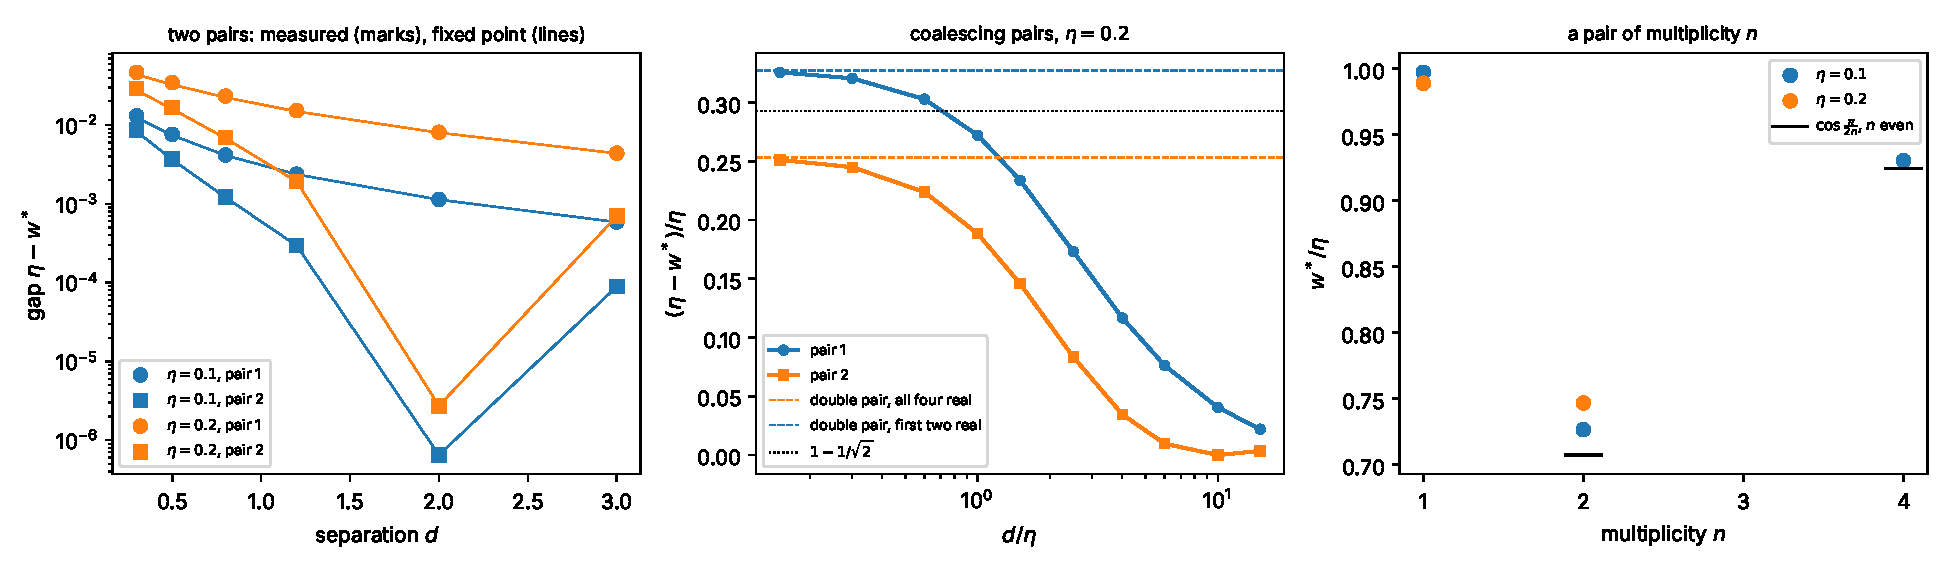
\includegraphics[width=\textwidth]{fig/cm_pairs.pdf}
\caption{Left: gaps of two planted pairs of equal width against their separation, by continuation (marks) and by the fixed point of Remark~\ref{cm:prop:gap} (lines). Centre: the gap over the width as two pairs of width $0.2$ coalesce, approaching the two stages of the double pair at this width (dashed), near the limit $1-1/\sqrt2$ (dotted). Right: the slice threshold of a pair of multiplicity $n$ over its width; for even $n$ it is close to $\cos\frac\pi{2n}$ (computed).}
\label{cm:fig:pairs}
\end{figure}

So the quantitative converse that one might hope for, ferromagnetism of $\cosh(wx)\,p$ implying no zero with $\re s>\frac12+w(1+o(1))$, fails by a constant factor already for double zeros: under Theorem~\ref{cm:thm:several}(ii) a double pair at distance $\delta$ from the line is invisible to the one variable test for every $w$ above about $\delta/\sqrt2$. For isolated clusters this is the worst case, since $\cos\frac\pi{2n}\ge\cos\frac\pi4$ for even $n$ and odd multiplicities have gaps of order $\eta^3$; whether some configuration of simple zeros does worse is part of Problem~\ref{cm:prob:interval}. The two spin system of Theorem~\ref{cm:thm:pair} has no such loss, which is one more reason to state the target in that form.

\section{A strip Lee and Yang theorem}\label{cm:sec:strip}

The Lee and Yang theorem says that a ferromagnetic coupling of spins in $\mathcal C_0$ gives a partition function with zeros only on the imaginary axis. For the strip classes the question is whether a coupling can widen the strip. It cannot, for symmetric spins whose Laplace transforms are of exponential type, by the general theorem of Lieb and Sokal.

\begin{theorem}\label{cm:thm:stripLY}
Let $\chi_1,\dots,\chi_N$ be symmetric probability measures on $\R$ whose Laplace transforms $\varphi_i(x)=\int e^{x\sigma}\chi_i(d\sigma)$ are entire of exponential type, for instance measures of bounded support, and suppose $\varphi_i(x)\ne0$ whenever $\re x>\delta_i$. Let $J_{ij}\ge0$. Then the partition function
\[
Z(h_1,\dots,h_N)=\int\exp\Big(\tfrac12\sum_{i,j}J_{ij}\sigma_i\sigma_j+\sum_ih_i\sigma_i\Big)\prod_i\chi_i(d\sigma_i)
\]
does not vanish when $\re h_i>\delta_i$ for every $i$. It does not vanish when $\re h_i<-\delta_i$ for every $i$ either, and in a common field all its zeros lie in $|\re h|\le\max_i\delta_i$.
\end{theorem}

\begin{proof}
$Z=\exp\big(\frac12\sum J_{ij}D_iD_j\big)\prod_i\varphi_i(x_i)$ at $x_i=h_i$, with $D_i=\partial/\partial x_i$. The function $G(x)=\prod_i\varphi_i(x_i+\delta_i)$ is entire of exponential type and does not vanish when every $\re x_i>0$. Since $\varphi_i$ is even, $\varphi_i(x)=\prod_k(1-x^2/r_{ik}^2)$ with $|\re r_{ik}|\le\delta_i$, so $G$ is the locally uniform limit of the polynomials $\prod_i\prod_{k\le n}(1-(x_i+\delta_i)^2/r_{ik}^2)$, which do not vanish when every $\re x_i>0$. By Proposition 2.2 of Lieb and Sokal \cite{LiebSokal81} and the domination argument of the proof of Theorem~\ref{cm:thm:stripXi}, $\exp(\frac12\sum J_{ij}D_iD_j)G$ does not vanish when every $\re x_i>0$; since translation commutes with the differential operator, that function is $Z(x_1+\delta_1,\dots,x_N+\delta_N)$. For $\re h_i<-\delta_i$ apply the same argument to the reflected measures.
\end{proof}

We have read Proposition 2.2 of \cite{LiebSokal81} in the restatement of \cite{NCLeeYang25}, not in the original. The theorem settles Problem~\ref{cm:prob:strip} as it was first posed for bounded spins, and it explains the computations of Figure~\ref{cm:fig:round3}, right: for spin one laws on $\{-1,0,1\}$ with $P(\pm1)=q<\frac14$, whose strip half width $a$ satisfies $\cosh a=\frac{1-2q}{2q}$, the strip of Curie Weiss systems and open chains of $2$, $4$ and $8$ spins never widens, shrinks monotonically with the coupling, and closes to $\mathcal C_0$ at a finite coupling. A random search over $1164$ systems with single spin laws on $\{-3,\dots,3\}$ found no widening, and $20000$ random tests of the multivariable form, a spin one law coupled to up to five Ising spins in independent complex fields, found no zero with $\re h_0>a$ when every Ising field has positive real part (computed). The shrinking is not part of the theorem.

\begin{figure}[htbp]
\centering
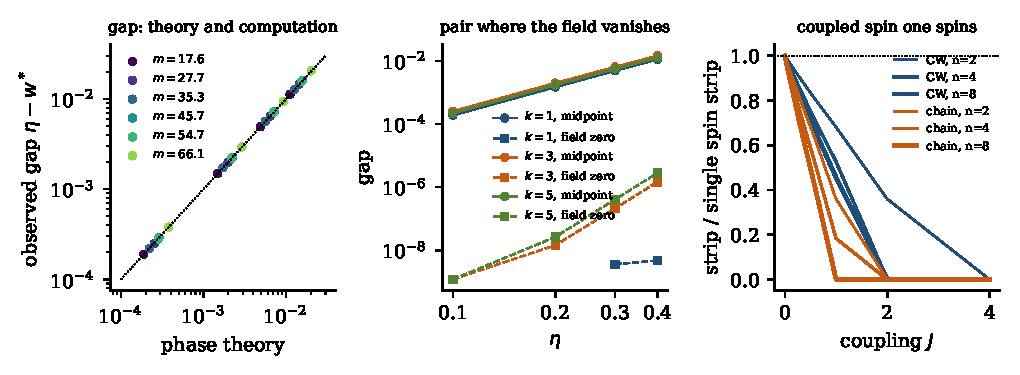
\includegraphics[width=\textwidth]{fig/cm_round3.pdf}
\caption{Left: the gap $\eta-w^*$ of Table~\ref{cm:tab:survey} against the phase theory of Remark~\ref{cm:prop:gap}. Centre: gaps for pairs planted at the midpoint and at the zero of the field $\phi$; at the zero of the field the gap is smaller by four to five orders of magnitude. Right: strip half width of coupled spin one spins, $q=0.2$, relative to one spin, against the coupling (computed).}
\label{cm:fig:round3}
\end{figure}

The P\'olya law is not of exponential type: its Laplace transform $\xi(\frac12+s)/\xi(\frac12)$ has order one and infinite type. The theorem still extends to it, for every ferromagnetic coupling, by approximating each transform with its truncated Hadamard products.

\begin{theorem}\label{cm:thm:stripXi}
Let $\chi_1,\dots,\chi_N$ be laws of Xi type with Gaussian moments of all orders, whose Laplace transforms satisfy $\varphi_i(x)\ne0$ for $\re x>\delta_i$, and let $J_{ij}\ge0$. Then $Z(h_1,\dots,h_N)\ne0$ whenever $\re h_i>\delta_i$ for every $i$. In particular $N$ P\'olya spins in any ferromagnetic coupling have all the zeros of their partition function in a common field in the strip $|\re h|\le\sup_\rho|\beta-\frac12|$, with no hypothesis.
\end{theorem}

\begin{proof}
With Gaussian moments of all orders $b=0$ in Definition~\ref{cm:def:X}, so $\varphi_i(x)=\prod_k(1-x^2/r_{ik}^2)$. Expanding $e^{\frac12\sigma\cdot J\sigma}$ in powers and integrating term by term, which Gaussian moments of all orders allow, gives $Z=\exp(\frac12\sum J_{ij}D_iD_j)\prod_i\varphi_i$ as a convergent series of derivatives. Let $\varphi_i^{(n)}(x)=\prod_{k\le n}(1-x^2/r_{ik}^2)$. These polynomials have their zeros among those of $\varphi_i$, so $\varphi_i^{(n)}(x)\ne0$ for $\re x>\delta_i$, and they converge to $\varphi_i$ locally uniformly. Their Taylor coefficients are bounded in modulus by those of $M_i(x)=\prod_k(1+x^2/|r_{ik}|^2)$, an entire function with nonnegative coefficients and $\log M_i(R)=o(R^2)$, because $\sum_k|r_{ik}|^{-2}<\infty$. Hence every term of the series for $Z^{(n)}=\exp(\frac12\sum J_{ij}D_iD_j)\prod_i\varphi_i^{(n)}$ at $h$ is bounded by the corresponding term of $\exp(\frac12\sum J_{ij}D_iD_j)\prod_iM_i$ at $(|h_1|,\dots,|h_N|)$. All terms of the latter are nonnegative and increase with the entries of $J$, so it is at most the same series for $J+cI$, which is positive semidefinite for $c$ large and is at most the Gaussian average $\E\prod_iM_i(|h_i|+|(\,(J+cI)^{1/2}\zeta)_i|)$, finite because $\log M_i(R)=o(R^2)$. By Tannery's theorem $Z^{(n)}\to Z$ locally uniformly on $\C^N$. By Proposition 2.2 of \cite{LiebSokal81} applied to the polynomial $\prod_i\varphi_i^{(n)}(x_i+\delta_i)$, each $Z^{(n)}$ is nonzero when $\re h_i>\delta_i$ for every $i$. By Hurwitz's theorem in several variables $Z$ is nowhere zero on that connected domain or identically zero there, and $Z>0$ for real $h$.
\end{proof}

This settles the extension asked for in the first version of Problem~\ref{cm:prob:strip}, for every nonnegative coupling and every law of Xi type with Gaussian moments of all orders, modulo the reading of Proposition 2.2 of \cite{LiebSokal81} noted above. As a check, two copies of the planted law of Proposition~\ref{cm:prop:counter}, with strip $0.3$, in the Curie Weiss coupling $a\begin{pmatrix}1&1\\1&1\end{pmatrix}$ have their zeros near the planted pair at real parts $0.300$, $0.293$, $0.265$, $0.229$ and $0.149$ for $a=0$, $0.002$, $0.01$, $0.02$ and $0.04$, and on the axis from $a=0.07$ on (computed, Gauss Hermite quadrature with 40 nodes): inside the strip, and moving towards the line. The bare pair coupling of the P\'olya spin with an Ising spin is the case below, where a direct proof is available.

\begin{proposition}\label{cm:prop:strippair}
Let $X$ be of Xi type in $\mathcal C_\delta$ and couple it to a fair Ising spin with strength $w\ge0$. In a common field $h$ the partition function $e^{h}L(h+w)+e^{-h}L(h-w)$ has no zero with $|\re h|>\delta$, and none off the imaginary axis when every zero of $L$ has $|\re r|<w$.
\end{proposition}

\begin{proof}
Let $h=y+iv$ with $y>\delta$. A zero $r$ of $L$ contributes $|h+w-r|/|h-w-r|$ to $|L(h+w)|/|L(h-w)|$, and $(y+w-\re r)^2-(y-w-\re r)^2=4w(y-\re r)\ge0$, with the partner $-r$ likewise; so $|L(h+w)|\ge|L(h-w)|$, while $|e^{h}|>|e^{-h}|$. Hence the two terms cannot cancel; $y<-\delta$ follows by symmetry. The second statement is Theorem~\ref{cm:thm:pair}(a) with $h_1=h_2=h$.
\end{proof}

For the descent the theorem is a monotonicity statement of the right kind: adding ferromagnetic interactions never moves zeros away from the line. It does not help with RH directly, because RH asks for an interaction to be removed.

\section{Approximation of the P\'olya density in Cauchy terms}\label{cm:sec:approx}

The ferromagnetic approximations of Section~\ref{ch:fmapprox}, whose best distance to the P\'olya law is $\operatorname{TV}<1.932\times10^{-6}$ with no hypothesis (Proposition~\ref{fm:prop:tvcert}), have a reading in this chapter. The zero completed law $f_K$ of Theorem~\ref{fm:thm:zc} has, by Theorem~\ref{cm:thm:signed}, the Thorin density
\[
u^{(K)}_y(v)=\frac{2\beta_K}\pi y+\sum_{k\le K}\big(P_y(v-\gamma_k)+P_y(v+\gamma_k)\big),\qquad\beta_K=\tfrac12\operatorname{Var}X-\sum_{k\le K}\gamma_k^{-2}.
\]
It keeps the first $K$ atoms of the mixing measure and replaces the rest by the drift. If the zeros above $\gamma_K$ are on the line, $0\le\frac{2\beta_K}\pi y-\sum_{k>K}2P_y(\gamma_k)\le\frac{2y^3}\pi\sum_{k>K}\gamma_k^{-4}$, so the drift is the low frequency limit of the far bumps (proved, conditional on the zeros above $\gamma_K$ only). At $y=\frac12$ the two Thorin densities agree at $v=0$ to within $4\times10^{-8}$ for $K=16$ and $5\times10^{-9}$ for $K=150$, and on $[0,\gamma_K/2]$ to within $6.3\times10^{-4}$ and $2.2\times10^{-4}$ (computed; Figure~\ref{cm:fig:fK}). Inside the ferromagnetic class the Thorin side is automatic once the atoms are real, and what must be proved is the positivity of the density, the dual of the deconvolution form of RH in Theorem~\ref{tf:thm:deconv}.

\begin{figure}[htbp]
\centering
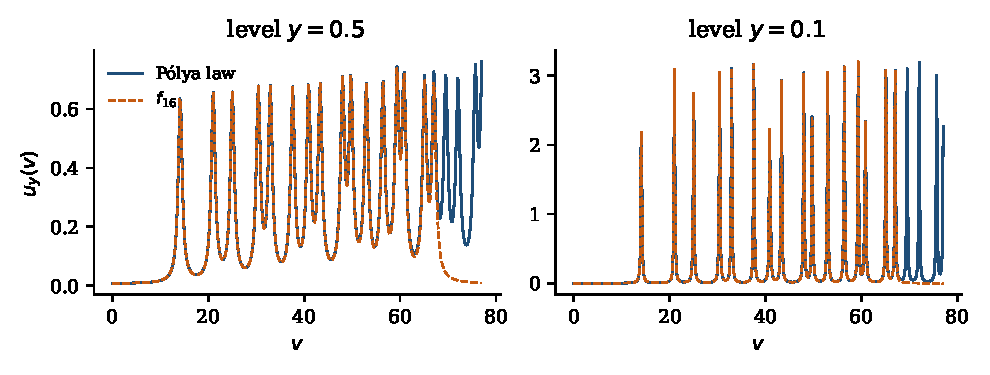
\includegraphics[width=\textwidth]{fig/cm_thorin_fK.pdf}
\caption{Thorin density of the P\'olya law (solid) and of the ferromagnetic law $f_{16}$ (dashed) at the levels $y=0.5$ and $y=0.1$; the approximant keeps sixteen bumps and replaces the rest by a constant (computed).}
\label{cm:fig:fK}
\end{figure}

\section{The target as monotonicity, and the function field model}\label{cm:sec:ff}

\begin{theorem}\label{cm:thm:mono}
The P\'olya spin coupled to one Ising spin is a Lee and Yang ferromagnet for every coupling $w>0$ if and only if $\sigma\mapsto|\xi(\sigma+it)|$ is nondecreasing on $[\frac12,\infty)$ for every $t$, if and only if RH holds.
\end{theorem}

\begin{proof}
By the proof of Theorem~\ref{cm:thm:pair} the Lee and Yang property at coupling $w$ implies $|L(h_1-w)|\le|L(h_1+w)|$ for $\re h_1>0$ (and is equivalent to it), and since $|L(-x+iv)|=|L(x+iv)|$ this reads $|L(|y-w|+iv)|\le|L(y+w+iv)|$ with $h_1=y+iv$. Taking $y=\frac{x_1+x_2}2$ and $w=\frac{x_2-x_1}2$ for $0\le x_1<x_2$ gives monotonicity of $|L(x+iv)|$ on $[0,\infty)$, and conversely. If $|L(\cdot+iv)|$ is nondecreasing and vanishes at $x_0>0$, it vanishes on $[0,x_0]$ and $L\equiv0$; so every zero is imaginary. Under RH each factor $|1-(x+iv)^2/r^2|$ with $r$ imaginary is nondecreasing in $x\ge0$.
\end{proof}

With strict increase this is the criterion of Sondow and Dumitrescu \cite{SD10}, and its infinitesimal form is Lagarias's \cite{Lagarias}. Lowering the coupling is shortening the horizontal segments across which $|\xi|$ must increase; at $w\ge\frac12$ they reach the line $\re s=1$, where the Euler product supplies the increase.

The function field case, where RH is a theorem, shows what a proof along this route needs. For an elliptic curve over $\mathbb F_q$ with $\#E(\mathbb F_q)=q+1-a$, the numerator of the zeta function gives, in $x=s-\frac12$,
\[
L_E(x)=q^x\big(1-aq^{-1/2-x}+q^{-2x}\big)=2\cosh(x\log q)-\frac a{\sqrt q}.
\]

\begin{proposition}\label{cm:prop:frob}
For $a\le0$, $L_E$ is the moment generating function of the three point measure with masses $1$, $|a|/\sqrt q$, $1$ at $-\log q$, $0$, $\log q$; for $a>0$ the imaginary field shift $x\mapsto x+i\pi/\log q$ turns it into minus such a function and changes no real part. Its zeros are imaginary if and only if $|a|\le2\sqrt q$, and otherwise lie at real parts $\pm\delta$, $\cosh(\delta\log q)=|a|/(2\sqrt q)$. Hence the Hasse bound holds exactly when this Frobenius spin is ferromagnetic, when its Thorin density is a single width Cauchy mixture at every level, and when the pair formed with an Ising spin is a Lee and Yang ferromagnet at every coupling.
\end{proposition}

\begin{proof}
$2\cosh z=e^z+e^{-z}$ and $\cosh(z+i\pi)=-\cosh z$; $\cosh(x\log q)=a/(2\sqrt q)$ has only imaginary solutions exactly when $|a|\le2\sqrt q$. The equivalences are Theorems~\ref{cm:thm:ferro} and~\ref{cm:thm:pair}, which use only the zeros.
\end{proof}

For a curve of genus $g$ the completed function is, when $|\alpha_j|=\sqrt q$, a product of $g$ factors $2\cosh(x\log q)-2\re(\alpha_j)/\sqrt q$, one Frobenius spin for each pair of eigenvalues. Hasse proved $|a|\le2\sqrt q$ from $\deg(m-n\pi)=m^2-amn+qn^2\ge0$, the nonnegativity of degrees of isogenies. In our language it is Weil positivity on two point test functions: for $g=m\delta_0-n\sqrt q\,\delta_{\log q}$ on the lattice $\log q\,\mathbb Z$, the sum of $|\widehat g|^2$ over the two zeros of one period is $2(m^2-amn+qn^2)$. The positivity comes from the geometry of the curve, not from the zeta function. For $y^2=x^3+x+1$ and the $165$ primes of good reduction among $5\le p<1000$ ($p=31$ is bad), $\max|a_p|/(2\sqrt p)=0.979$, so every Frobenius spin is ferromagnetic; a fake factor with $|a|/(2\sqrt q)=1.3$ at $q=101$ has strip $\delta=0.164$ and a Thorin density that is negative below it (Figure~\ref{cm:fig:curves}; computed).

\begin{figure}[htbp]
\centering
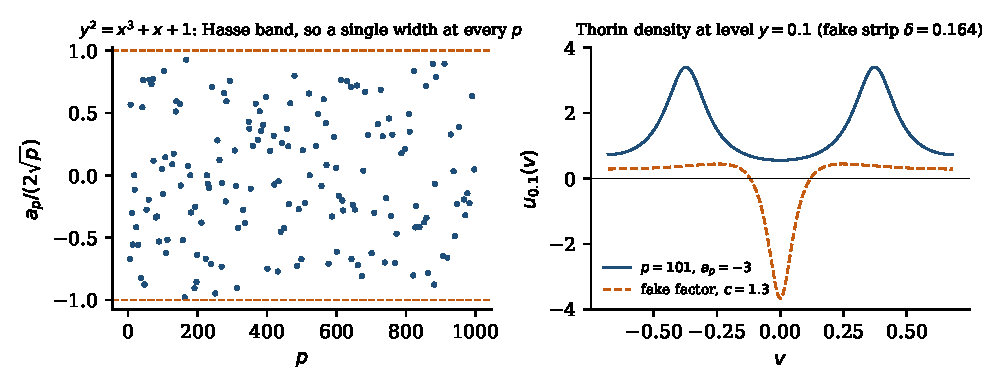
\includegraphics[width=\textwidth]{fig/cm_curves.pdf}
\caption{Left: normalised Frobenius traces $a_p/(2\sqrt p)$ of $y^2=x^3+x+1$ for $p<1000$, all inside the Hasse band. Right: Thorin density at level $y=0.1$ of the genuine factor at $p=101$ and of a fake factor beyond the Hasse bound (computed).}
\label{cm:fig:curves}
\end{figure}

The comparison locates the gap exactly. A curve has finitely many Frobenius spins, each of exponential type, so for the Frobenius spins that are laws (a spin with $a>0$ is a signed measure) the Lee and Yang theory of Theorem~\ref{cm:thm:stripLY} applies, and a finite computation decides each curve; the positivity that makes the spins ferromagnetic comes from intersection theory. The P\'olya spin is one spin of infinite type, the Maxwell decomposition of Theorem~\ref{fm:thm:maxwell} into infinitely many ferromagnetic spins is RH itself, and no source of positivity outside $\zeta$ is known. A proof along this route needs a positive form, built from the primes, whose diagonal values are the Weil functional; that is the Hilbert and P\'olya problem in the language of ferromagnets.

\section{A Fej\'er window at level $\frac12+\delta$ and the height test}\label{cm:sec:window}

This section records the explicit formula for a Cauchy times Fej\'er window, a test for off line zeros at level one that needs no bound on the interference of the other zeros, its ceiling, and a heuristic for the resolution. It is the finite window version of the damped criterion (Theorem~\ref{dc:thm:damped}) and of the Cauchy smoothed measure of Remark~\ref{bsy:rem:weil}.

For $\delta>0$ and $L>0$ let $G(x)=e^{-\delta|x|}(1-|x|/L)_+$, with transform $H$, and for a centre $w$ let $g_w(x)=G(x)\cos wx$, whose transform is $h_w(r)=\frac12[H(r-w)+H(r+w)]$. The function $G$ is even, Lipschitz, of compact support, with $G'$ of bounded variation, so $\widehat{g_w}$ lies in the class $\mathcal B$ of Theorem~\ref{dc:thm:weil}; this hypothesis is needed, since the explicit formula fails for an even compactly supported function that is not regular enough (the indicator of an interval, whose transform decays like $1/r$). The flow $O_{\delta,L}(w)$ is the right side of the explicit formula for $g_w$, namely the archimedean and pole terms minus $2\sum_{n\le e^L}\Lambda(n)n^{-1/2-\delta}(1-\log n/L)\cos(w\log n)$; the prime part enters with a minus sign.

\begin{theorem}[finite prime side at every level]\label{cm:thm:flow}
For every $\delta>0$ and $L>0$, unconditionally, $O_{\delta,L}(w)=\sum_\rho h_w(\gamma_\rho)$, the series converging absolutely, and the prime side contains only the prime powers $n\le e^L$. Status: proved.
\end{theorem}

\begin{proof}
This is Theorem~\ref{dc:thm:weil} for $g_w$, whose support is $[-L,L]$.
\end{proof}

The identity computes the Cauchy smoothed measure of Remark~\ref{bsy:rem:weil} further smoothed by the Fej\'er kernel, and the truncation reappears as a bias: the peak of one isolated zero on the line has height $H(0)=2/\delta-2(1-e^{-\delta L})/(\delta^2L)$, which is $11.55$ against $2/\delta=40$ at $\delta=0.05$, $L=14.5087$ (proved for the formula, computed for the numbers). The limit $L\to\infty$ gives the Cauchy smoothed measure $2v_{1/2+\delta}$ if every zero has $|\beta-\frac12|<\delta$ (proved, by dominated convergence, the pair kernels being bounded by $C(\delta)/r^2$ uniformly in $L\ge1$). If some zero has $\eta=|\beta-\frac12|>\delta$, its pair term is of size $e^{(\eta-\delta)L}/(L((\eta-\delta)^2+u^2))$ at distance $u$, with a sign that depends on $uL$, and the limit does not exist.

\begin{theorem}[height test at level one]\label{cm:thm:height}
Let $G$ be even, $G(0)=1$, $G\ge0$, supported in $[-L,L]$, with $\widehat{g_w}\in\mathcal B$, and such that $G(x)\cosh(\eta x)$ is positive definite for every $\eta\in[0,\frac12)$. Examples are $e^{-|x|/2}(1-|x|/L)_+$ and $\operatorname{sech}(x/2)(1-|x|/L)_+$. Let $O(w)$ be the flow of $G$ and $H_0(0)=\int G$. If $\sup_{w\in I}O(w)<2H_0(0)$ on an interval $I$, then every zero of $\zeta$ with ordinate in $I$ is simple and on the critical line. Status: proved.
\end{theorem}

\begin{proof}
Since $\zeta$ has no zero on $\Re s=1$, every zero has $\eta<\frac12$. Group the zeros in orbits under $\rho\mapsto1-\bar\rho$, which preserve the ordinate. A zero on the line contributes $H_0(w-\gamma)+H_0(w+\gamma)\ge0$, and an off line pair contributes $2H_\eta(w-\gamma)+2H_\eta(w+\gamma)\ge0$, where $H_\eta$ is the transform of $G\cosh\eta x$; so $O(w)$ dominates every single orbit. At $w=\gamma$ an off line pair gives at least $2H_\eta(0)\ge2H_0(0)$ since $\cosh\ge1$, and so does a double zero on the line. The positivity: $e^{-|x|/2}\cosh\eta x$ is half the sum of $e^{-(1/2\mp\eta)|x|}$; the transform of $\operatorname{sech}(x/2)\cosh\eta x$ is $4\pi\cos(\pi\eta)\cosh(\pi r)/(\cosh2\pi r+\cos2\pi\eta)>0$; and multiplication by the Fej\'er triangle keeps positive definiteness.
\end{proof}

No bound on the interference is needed, because it has a sign. In substance this is the positivity behind de la Vall\'ee Poussin's argument (Theorem~\ref{cf:thm:dvp}), used as a test on a window of ordinates; it uses the nonvanishing of $\zeta$ on $\Re s=1$, which is the Euler product, and it does not transfer to the Davenport and Heilbronn function, which has zeros with $\beta>1$.

How far the test reaches is a computation. With $G=e^{-|x|/2}(1-|x|/L)_+$ ($\delta=\frac12$) and $L=14.51$ the maximum of $O/H_0(0)$ over ordinates in $[5,160]$ is $1.5085<2$, so the zeros there are simple and on the line (computed, double precision, on a grid of step $0.01$; a bound between grid nodes needs ball arithmetic, which has not been run). With the sech kernel and the primes below $2\times10^6$ the first ordinate $w$ with $O(w)\ge2H_0(0)$ is $1329.03$ (computed, same caveats); the stop is the close pair of zeros at $1329.04$ and $1329.21$, whose gap is below the width of the kernel. This is exclusion on a window, and no alternative to Turing's method.

\begin{theorem}[ceiling of the test]\label{cm:thm:ceiling}
For any $G$ as in Theorem~\ref{cm:thm:height} one has $G\le\operatorname{sech}(x/2)$ and $H_0(0)\le2\pi$, and the hypothesis $\sup_IO<2H_0(0)$ on a window $I=[T,T+W]$ with $W\ge W_0(G)$ can hold only if $\log(T/2\pi)<4\pi$, that is $T<2\pi e^{4\pi}\approx1.8\times10^6$. If it is known a priori that all zeros satisfy $|\beta-\frac12|\le\eta_0$, the same argument with $G\cosh\eta_0x$ gives $H_0(0)\le\pi/\eta_0$ and the necessary condition $\eta_0<2\pi/\log(T/2\pi)$. Status: proved.
\end{theorem}

\begin{proof}
Positive definiteness of $G\cosh\eta x$ gives $|G(x)\cosh\eta x|\le1$, hence $G\le\operatorname{sech}(x/2)$ and $H_0(0)\le2\pi$. Over a long window near $T$ the mean of $O$ is $\log(T/2\pi)+o(1)$: the prime cosines average to zero at fixed $L$, the pole term tends to $0$, and the archimedean term with $-\log\pi$ gives $\log(w/2\pi)$ since $G(0)=1$. So $\sup O\ge\log(T/2\pi)-o(1)$ as $W\to\infty$, and $\sup O<2H_0(0)<4\pi$, strictly since $G$ has compact support, forces the stated bound for $W\ge W_0(G)$. The strip form is the same with $\cosh\eta_0x$.
\end{proof}

So the positivity route at height $T$ needs a zero free region reaching to within $2\pi/\log(T/2\pi)$ of the line from the right, whereas the known regions start from $\Re s=1$, with width $c/\log T$ or the Vinogradov Korobov width; the gap is the whole strip.

\begin{proposition}[size of the interference below level one]\label{cm:prop:nt}
Let $\delta<\frac12$. A pair with $\eta>\delta$ at distance $d$ from the centre contributes about $2e^{(\eta-\delta)L}/(L((\eta-\delta)^2+d^2))$, with a sign that depends on $dL$. The counting function $N(T)$ does not see $\eta$, and without RH the only a priori limit is $\eta<\frac12$, so a bound on the interference from $N(T)$ alone is at least of order $e^{(1/2-\delta)L}/(Ld^2)$, against $H(0)\le L$. Status: proved as a size statement; the Davenport and Heilbronn function, which has a functional equation of the same shape, realises it (computed).
\end{proposition}

For that function the pair at $240.40$ contributes, at distance $5.03$ and $\delta=0.05$, $-0.02$, $+0.035$, $-0.155$ and $-1.93$ in units of $H(0)$ for $L=10,14.5,20,30$ (computed). Resolving zeros near $T$ needs $L$ of order $2\log(T/2\pi)$, so no argument that uses only properties shared with that function, in particular one from $N(T)$, can give a bound for $\delta<\frac12$.

\begin{remark}[resolution law, heuristic]\label{cm:rem:resolution}
Let $g$ be the gap to the neighbouring zero. Reading a zero needs $L\ge2\pi/g$ and the primes up to $e^L$, which is the heuristic $\Omega=\pi/\delta$ of Remark~\ref{es:rem:resolution}. For the zeros below $8148$ with $\delta=1/L$ the $L$ that reads $90$ per cent of the zeros in a window near $T$ is $1.7$ to $2.0$ times $\log(T/2\pi)$ (computed), and the $L$ that reads every zero is $2\pi/g_{\min}(T)$ (computed). Extrapolated with $L=1.9\log(T/2\pi)$ for $90$ per cent and $e^L/L$ primes (heuristic):
\begin{center}\small
\begin{tabular}{rrrr}
$T$ & $\log(T/2\pi)$ & $L$ & primes \\
\hline
$150$ & $3.2$ & $6$ & $70$ \\
$10^4$ & $7.4$ & $14$ & $9\times10^4$ \\
$10^6$ & $12.0$ & $23$ & $3\times10^8$ \\
$3\times10^{12}$ & $26.9$ & $51$ & $3\times10^{20}$ \\
\end{tabular}
\end{center}
At $T=3\times10^{12}$ the primes up to $(T/2\pi)^{1.9}$ are about $3\times10^{20}$, against about $T^{1/2}$ terms for a value of $\zeta$ by the Riemann Siegel formula. Deconvolution therefore has no height limit in principle, since the identity of Theorem~\ref{cm:thm:flow} holds at every height, and a severe one in practice: the cost grows faster than any power of $T$ for all zeros, the proof that a peak is a zero on the line stops at the ceiling of Theorem~\ref{cm:thm:ceiling}, and below $\delta=\frac12$ it is lost by Proposition~\ref{cm:prop:nt}.
\end{remark}

\begin{remark}[control]\label{cm:rem:dh}
For the Davenport and Heilbronn function (explicit formula with conductor $5$) the flow with $\delta=0.05$ and the primes $n\le500$ ($L=6.2$) has, among its maxima with $O/H(0)$ at least $2$, exactly the five off line ordinates below $300$ (about $85.70$, $114.16$, $166.48$, $176.70$, $240.40$), read to $0.01$, and this stays so to $n=3\times10^5$ (computed). At $\delta=\frac12$ the maxima above $2$ at $n=10^4$ include on line clusters (for example near $145.44$ and $149.38$), because the conductor raises the background, which is consistent with Theorem~\ref{cm:thm:height} being a one way statement. A pass at $\delta<\frac12$ says little; a negative value of the flow, if every $|\eta|\le\delta$ would give $O\ge0$, proves a zero with $|\eta|>\delta$ (Theorem~\ref{dc:thm:damped}).
\end{remark}

\section{Is this a path to RH?}\label{cm:sec:path}

No. The four forms of RH in this chapter, the single width Cauchy mixture, the ferromagnetism of the P\'olya law, Weil's functional and the Lee and Yang property of the two spin system at every coupling, are each proved at the level one or the coupling $\frac12$, and each step below is a zero free half plane (Corollary~\ref{cm:cor:pair}). The descent in coupling is the descent in level of Section~\ref{ov1:sec:path}, and the three constraints apply. A proof must be infinite, since finite Euler products sit at $w=\frac12$ (Proposition~\ref{cm:prop:euler}) and finite computations cannot exclude zeros above them (Theorem~\ref{thm:ch13:perturb}). It must use the Euler product, since the Davenport and Heilbronn function has the same Cauchy structure. And it must not rest on a property preserved by Gaussian damping (Corollary~\ref{cm:cor:emn}). In statistical mechanical terms the Lee and Yang property is preserved when ferromagnetic interactions are added and RH asks for one to be removed, the coupling to the Ising spin; no general theorem goes in that direction, and $\Lambda\ge0$ says that the self interaction of the de Bruijn Newman flow cannot be removed either. What the chapter adds is the exact form of the target and the fact that the natural one variable test is strictly weaker than it.

\section{Open problems}\label{cm:sec:open}

\begin{problem}\label{cm:prob:interval}
For the one variable tilt, is the set of $w$ for which $\cosh(wx)\,P(dx)$ is ferromagnetic always an interval? Theorems~\ref{cm:thm:exact} and~\ref{cm:thm:several} treat clusters that are small compared with their distance from the other zeros. Extend the gap law to clusters whose width is comparable to the spacing of the neighbouring zeros, where the fixed point of Remark~\ref{cm:prop:gap} is still accurate (Table~\ref{cm:tab:pairs}) but no theorem applies. Is there a constant $\kappa>0$ such that ferromagnetism of $\cosh(wx)\,P(dx)$ for every $w>w_0$ implies that no zero has $|\re r|>w_0/\kappa$? Proposition~\ref{cm:prop:twospin} gives $\kappa\le\cos\frac\pi4$: its law is ferromagnetic for every $w>w_0$ exactly when $w_0\ge w^*$ and has a zero with $|\re r|=a$, so $\kappa\le w^*/a$, which tends to $\cos\frac\pi4$ as $q\uparrow\frac14$.
\end{problem}

\begin{problem}\label{cm:prob:euler}
Find a coupled system of Lee and Yang spins built from the Euler product, not from $\xi$, with coupling below $\frac12$ and a partition function that contains $L(h_1\pm w)$; by Corollary~\ref{cm:cor:pair} its Lee and Yang property would be a zero free half plane.
\end{problem}

\begin{problem}\label{cm:prob:strip}
Theorem~\ref{cm:thm:stripXi} shows that ferromagnetic couplings never widen the strip. Do they shrink it strictly, by at least an amount comparable to the coupling, as the computations of Section~\ref{cm:sec:strip} suggest? A quantitative shrinking theorem for a coupling that can be removed again would be new information about a single spin.
\end{problem}
